\section{Solved Problems}


\begin{problem}[A $ C^\infty $ atlas on a circle (From W. Tu)]
	\label{problem:AtlasForCircleComplexPlane}
	construct a $ C^\infty $ atlas for the unit circle $ S^1 $. 
\end{problem}
\begin{solution}
	The unit circle $ C^1 $ can be described as a set of points $ S^1 =  \set{e^{it}| t \in [0,2\pi]} $. Let $ U_1 $ and $ U_2 $ be two subsets of $ S^1 $ described as
	\[ U_1 = \set{e^{it}| t \in (-\pi,\pi)},\qquad U_2 = \set{e^{it}| t \in (0,2\pi)}. \]
	Consider the functions $ \phi_\alpha: U_\alpha \to \R $ for $ \alpha = 1,2 $ given by
	\begin{align*}
		&\phi_1(e^{it}) = t, \qquad -\pi<t<\pi,\\
		&\phi_2(e^{it}) = t, \qquad 0<t<2\pi.
	\end{align*}
	These functions are in fact different branches of the complex logarithm function $ 1/i\log(z) $, thus homeomorphisms onto their respective images. Thus $ \set{(U_1,\phi_1),(U_2,\phi_2)} $ is an atlas for $ S^1 $. To demonstrate the compatibility of these charts, we need to first calculate $ U_1 \cap U_2 $. This set has two connected components, i.e. $ U_1 \cap U_2 = A \sqcup B $ where $ \sqcup $ is used to demonstrate the disjoint union of $ A,B $. Explicitly, we can write
	\[ A = \set{e^{it}| t \in (-\pi,0)}, \qquad B = \set{e^{it}| t\in(0,\pi)}. \]
	First, we start with the function $ \phi_1 \circ \phi_2^{-1}: \underbrace{\phi_2(U_1\cap U_2)}_{(0,\pi)\sqcup (\pi,2\pi)} \to \underbrace{\phi_1(U_1\cap U_2)}_{(-\pi,0)\sqcup (0,\pi)} $. For this function we have
	\[ (\phi_1\circ\phi_2^{-1})(t) = \begin{cases}
		t \qquad &t\in(0,\pi),\\
		t - 2\pi \qquad &t\in(\pi,2\pi).
	\end{cases} \]
	Similarly, for $ \phi_2 \circ \phi_1^{-1}: \underbrace{\phi_1(U_1\cap U_2)}_{(-\pi,0)\sqcup (0,\pi)} \to \underbrace{\phi_2(U_1\cap U_2)}_{(0,\pi)\sqcup (\pi,2\pi)} $ we can write
	\[ (\phi_2\circ\phi_1^{-1})(t) = \begin{cases}
		t+2\pi \qquad &t\in(0,\pi),\\
		t \qquad &t\in(\pi,2\pi).
	\end{cases} \]
	\begin{figure}[h!]
	\centering

	
	
	\tikzset{every picture/.style={line width=0.75pt}} %set default line width to 0.75pt        
	
	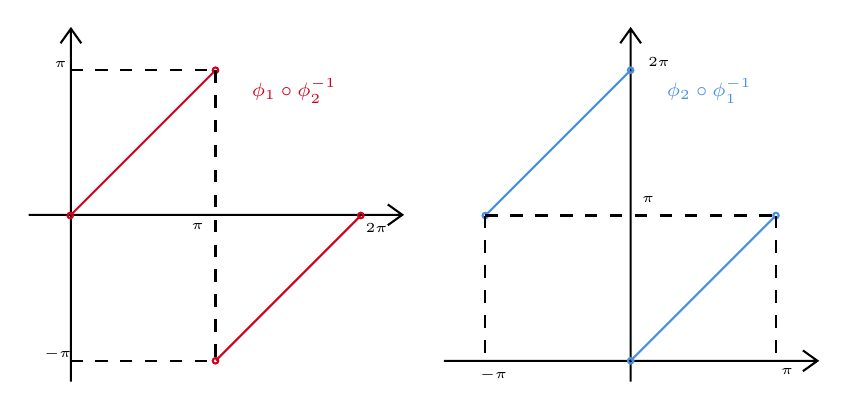
\begin{tikzpicture}[x=0.75pt,y=0.75pt,yscale=-1,xscale=1]
		%uncomment if require: \path (0,300); %set diagram left start at 0, and has height of 300
		
		%Shape: Axis 2D [id:dp031269396086308854] 
		\draw  (180,189.67) -- (360,189.67)(200.33,100) -- (200.33,270) (353,184.67) -- (360,189.67) -- (353,194.67) (195.33,107) -- (200.33,100) -- (205.33,107)  ;
		%Straight Lines [id:da8173483474090752] 
		\draw [color={rgb, 255:red, 208; green, 2; blue, 27 }  ,draw opacity=1 ][line width=0.75]    (200.24,189.76) -- (269.76,120.24) ;
		\draw [shift={(270,120)}, rotate = 315] [color={rgb, 255:red, 208; green, 2; blue, 27 }  ,draw opacity=1 ][line width=0.75]      (0, 0) circle [x radius= 1.34, y radius= 1.34]   ;
		\draw [shift={(200,190)}, rotate = 315] [color={rgb, 255:red, 208; green, 2; blue, 27 }  ,draw opacity=1 ][line width=0.75]      (0, 0) circle [x radius= 1.34, y radius= 1.34]   ;
		%Straight Lines [id:da7972743834901372] 
		\draw [color={rgb, 255:red, 208; green, 2; blue, 27 }  ,draw opacity=1 ][line width=0.75]    (270.24,259.76) -- (339.76,190.24) ;
		\draw [shift={(340,190)}, rotate = 315] [color={rgb, 255:red, 208; green, 2; blue, 27 }  ,draw opacity=1 ][line width=0.75]      (0, 0) circle [x radius= 1.34, y radius= 1.34]   ;
		\draw [shift={(270,260)}, rotate = 315] [color={rgb, 255:red, 208; green, 2; blue, 27 }  ,draw opacity=1 ][line width=0.75]      (0, 0) circle [x radius= 1.34, y radius= 1.34]   ;
		%Straight Lines [id:da11749218813373297] 
		\draw  [dash pattern={on 4.5pt off 4.5pt}]  (270,120) -- (270,260) ;
		%Shape: Axis 2D [id:dp7242837319994968] 
		\draw  (380,260) -- (560,260)(470,100) -- (470,270) (553,255) -- (560,260) -- (553,265) (465,107) -- (470,100) -- (475,107)  ;
		%Straight Lines [id:da7954245800299584] 
		\draw [color={rgb, 255:red, 74; green, 144; blue, 226 }  ,draw opacity=1 ][line width=0.75]    (400.24,189.76) -- (469.76,120.24) ;
		\draw [shift={(470,120)}, rotate = 315] [color={rgb, 255:red, 74; green, 144; blue, 226 }  ,draw opacity=1 ][line width=0.75]      (0, 0) circle [x radius= 1.34, y radius= 1.34]   ;
		\draw [shift={(400,190)}, rotate = 315] [color={rgb, 255:red, 74; green, 144; blue, 226 }  ,draw opacity=1 ][line width=0.75]      (0, 0) circle [x radius= 1.34, y radius= 1.34]   ;
		%Straight Lines [id:da15608839189923596] 
		\draw [color={rgb, 255:red, 74; green, 144; blue, 226 }  ,draw opacity=1 ][line width=0.75]    (470.24,259.76) -- (539.76,190.24) ;
		\draw [shift={(540,190)}, rotate = 315] [color={rgb, 255:red, 74; green, 144; blue, 226 }  ,draw opacity=1 ][line width=0.75]      (0, 0) circle [x radius= 1.34, y radius= 1.34]   ;
		\draw [shift={(470,260)}, rotate = 315] [color={rgb, 255:red, 74; green, 144; blue, 226 }  ,draw opacity=1 ][line width=0.75]      (0, 0) circle [x radius= 1.34, y radius= 1.34]   ;
		%Straight Lines [id:da8863860410352722] 
		\draw  [dash pattern={on 4.5pt off 4.5pt}]  (400,190) -- (400,260) ;
		%Straight Lines [id:da8092780134149673] 
		\draw  [dash pattern={on 4.5pt off 4.5pt}]  (540,190) -- (540,260) ;
		%Straight Lines [id:da9907647632614371] 
		\draw  [dash pattern={on 4.5pt off 4.5pt}]  (400,190) -- (540,190) ;
		%Straight Lines [id:da6719155425075689] 
		\draw  [dash pattern={on 4.5pt off 4.5pt}]  (200,260) -- (270,260) ;
		%Straight Lines [id:da26461137148185054] 
		\draw  [dash pattern={on 4.5pt off 4.5pt}]  (200,120) -- (270,120) ;
		
		% Text Node
		\draw (257,192.4) node [anchor=north west][inner sep=0.75pt]  [font=\tiny]  {$\pi $};
		% Text Node
		\draw (286,122.4) node [anchor=north west][inner sep=0.75pt]  [font=\scriptsize,color={rgb, 255:red, 208; green, 2; blue, 27 }  ,opacity=1 ]  {$\phi _{1} \circ \phi _{2}^{-1}$};
		% Text Node
		\draw (341,192.4) node [anchor=north west][inner sep=0.75pt]  [font=\tiny]  {$2\pi $};
		% Text Node
		\draw (396,262.4) node [anchor=north west][inner sep=0.75pt]  [font=\tiny]  {$-\pi $};
		% Text Node
		\draw (486,122.4) node [anchor=north west][inner sep=0.75pt]  [font=\scriptsize,color={rgb, 255:red, 74; green, 144; blue, 226 }  ,opacity=1 ]  {$\phi _{2} \circ \phi _{1}^{-1}$};
		% Text Node
		\draw (541,262.4) node [anchor=north west][inner sep=0.75pt]  [font=\tiny]  {$\pi $};
		% Text Node
		\draw (474,179.4) node [anchor=north west][inner sep=0.75pt]  [font=\tiny]  {$\pi $};
		% Text Node
		\draw (477,112.4) node [anchor=north west][inner sep=0.75pt]  [font=\tiny]  {$2\pi $};
		% Text Node
		\draw (191,114.4) node [anchor=north west][inner sep=0.75pt]  [font=\tiny]  {$\pi $};
		% Text Node
		\draw (186,252.4) node [anchor=north west][inner sep=0.75pt]  [font=\tiny]  {$-\pi $};
		
		
	\end{tikzpicture}
\end{figure}
	
\end{solution}

\begin{observation}
	I was thinking about my solution to the problem above, and I thought it is wrong, as I was thinking that the function $ \phi_1 $ is not homeomorphism as it is not continuous. But the point that I was missing is that this function is indeed continuous on its domain and the point of discontinuity (i.e. $ x = \pi $) is not in the domain. 
\end{observation}

\begin{problem}{Another $ C^\infty $ atlas on a circle}
	\label{problem:S^1Charts}
	In the previous problem, we constructed an atlas for a unit circle siting in the complex plane. In this problem we are going to construct a different atlas for a unit circle siting in the $ x-y $ plane. The following diagram are the charts for this unit circle. Write these charts explicitly and check if they are pairwise compatible.
	\begin{figure}[h!]
	
	
	\centering
	\tikzset{every picture/.style={line width=0.75pt}} %set default line width to 0.75pt        
	
	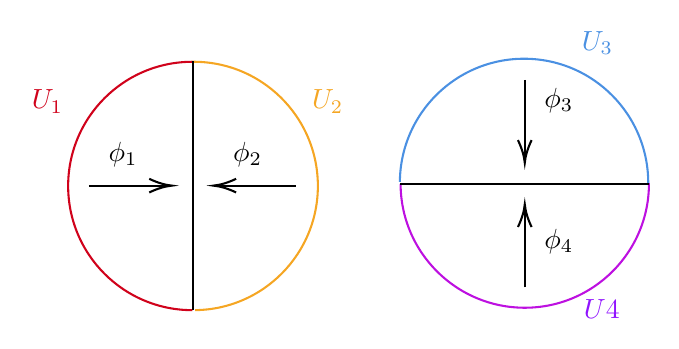
\begin{tikzpicture}[x=0.75pt,y=0.75pt,yscale=-1,xscale=1]
		%uncomment if require: \path (0,300); %set diagram left start at 0, and has height of 300
		
		%Shape: Arc [id:dp023481932229717062] 
		\draw  [draw opacity=0] (199.83,250) .. controls (199.83,250) and (199.83,250) .. (199.83,250) .. controls (199.83,250) and (199.83,250) .. (199.83,250) .. controls (166.79,250) and (140,223.21) .. (140,190.17) .. controls (140,157.12) and (166.79,130.33) .. (199.83,130.33) -- (199.83,190.17) -- cycle ; \draw  [color={rgb, 255:red, 208; green, 2; blue, 27 }  ,draw opacity=1 ] (199.83,250) .. controls (199.83,250) and (199.83,250) .. (199.83,250) .. controls (199.83,250) and (199.83,250) .. (199.83,250) .. controls (166.79,250) and (140,223.21) .. (140,190.17) .. controls (140,157.12) and (166.79,130.33) .. (199.83,130.33) ;  
		%Shape: Arc [id:dp8279857043077765] 
		\draw  [draw opacity=0] (199.83,130.33) .. controls (199.83,130.33) and (199.83,130.33) .. (199.83,130.33) .. controls (232.88,129.98) and (259.95,156.47) .. (260.31,189.52) .. controls (260.67,222.56) and (234.17,249.64) .. (201.13,249.99) -- (200.48,190.16) -- cycle ; \draw  [color={rgb, 255:red, 245; green, 166; blue, 35 }  ,draw opacity=1 ] (199.83,130.33) .. controls (199.83,130.33) and (199.83,130.33) .. (199.83,130.33) .. controls (232.88,129.98) and (259.95,156.47) .. (260.31,189.52) .. controls (260.67,222.56) and (234.17,249.64) .. (201.13,249.99) ;  
		%Shape: Arc [id:dp2277450931666709] 
		\draw  [draw opacity=0] (299.82,188.21) .. controls (299.82,188.21) and (299.82,188.21) .. (299.82,188.21) .. controls (300.08,155.16) and (327.08,128.59) .. (360.13,128.86) .. controls (393.17,129.12) and (419.75,156.12) .. (419.48,189.17) -- (359.65,188.69) -- cycle ; \draw  [color={rgb, 255:red, 74; green, 144; blue, 226 }  ,draw opacity=1 ] (299.82,188.21) .. controls (299.82,188.21) and (299.82,188.21) .. (299.82,188.21) .. controls (300.08,155.16) and (327.08,128.59) .. (360.13,128.86) .. controls (393.17,129.12) and (419.75,156.12) .. (419.48,189.17) ;  
		%Shape: Arc [id:dp16056893747855794] 
		\draw  [draw opacity=0] (419.83,188.83) .. controls (419.83,188.83) and (419.83,188.83) .. (419.83,188.83) .. controls (419.93,221.88) and (393.21,248.74) .. (360.17,248.83) .. controls (327.12,248.93) and (300.26,222.21) .. (300.17,189.17) -- (360,189) -- cycle ; \draw  [color={rgb, 255:red, 189; green, 16; blue, 224 }  ,draw opacity=1 ] (419.83,188.83) .. controls (419.83,188.83) and (419.83,188.83) .. (419.83,188.83) .. controls (419.93,221.88) and (393.21,248.74) .. (360.17,248.83) .. controls (327.12,248.93) and (300.26,222.21) .. (300.17,189.17) ;  
		%Straight Lines [id:da9947609889928073] 
		\draw    (150,190) -- (188,190) ;
		\draw [shift={(190,190)}, rotate = 180] [color={rgb, 255:red, 0; green, 0; blue, 0 }  ][line width=0.75]    (10.93,-3.29) .. controls (6.95,-1.4) and (3.31,-0.3) .. (0,0) .. controls (3.31,0.3) and (6.95,1.4) .. (10.93,3.29)   ;
		%Straight Lines [id:da6553860547904606] 
		\draw    (212,190) -- (250,190) ;
		\draw [shift={(210,190)}, rotate = 0] [color={rgb, 255:red, 0; green, 0; blue, 0 }  ][line width=0.75]    (10.93,-3.29) .. controls (6.95,-1.4) and (3.31,-0.3) .. (0,0) .. controls (3.31,0.3) and (6.95,1.4) .. (10.93,3.29)   ;
		%Straight Lines [id:da19474028508083085] 
		\draw    (360,139) -- (360,177) ;
		\draw [shift={(360,179)}, rotate = 270] [color={rgb, 255:red, 0; green, 0; blue, 0 }  ][line width=0.75]    (10.93,-3.29) .. controls (6.95,-1.4) and (3.31,-0.3) .. (0,0) .. controls (3.31,0.3) and (6.95,1.4) .. (10.93,3.29)   ;
		%Straight Lines [id:da648683487634115] 
		\draw    (360,239) -- (360,201) ;
		\draw [shift={(360,199)}, rotate = 90] [color={rgb, 255:red, 0; green, 0; blue, 0 }  ][line width=0.75]    (10.93,-3.29) .. controls (6.95,-1.4) and (3.31,-0.3) .. (0,0) .. controls (3.31,0.3) and (6.95,1.4) .. (10.93,3.29)   ;
		%Straight Lines [id:da9130830416071034] 
		\draw    (200,130) -- (200,250) ;
		%Straight Lines [id:da1322223309435544] 
		\draw    (420,189) -- (300,189) ;
		
		% Text Node
		\draw (121,142.4) node [anchor=north west][inner sep=0.75pt]  [color={rgb, 255:red, 208; green, 2; blue, 27 }  ,opacity=1 ]  {$U_{1}$};
		% Text Node
		\draw (256,142.4) node [anchor=north west][inner sep=0.75pt]  [color={rgb, 255:red, 245; green, 166; blue, 35 }  ,opacity=1 ]  {$U_{2}$};
		% Text Node
		\draw (386,114.4) node [anchor=north west][inner sep=0.75pt]  [color={rgb, 255:red, 74; green, 144; blue, 226 }  ,opacity=1 ]  {$U_{3}$};
		% Text Node
		\draw (387,243.4) node [anchor=north west][inner sep=0.75pt]  [color={rgb, 255:red, 144; green, 19; blue, 254 }  ,opacity=1 ]  {$U4$};
		% Text Node
		\draw (158,167.4) node [anchor=north west][inner sep=0.75pt]    {$\phi _{1}$};
		% Text Node
		\draw (218,167.4) node [anchor=north west][inner sep=0.75pt]    {$\phi _{2}$};
		% Text Node
		\draw (368,141.4) node [anchor=north west][inner sep=0.75pt]    {$\phi _{3}$};
		% Text Node
		\draw (368,209.4) node [anchor=north west][inner sep=0.75pt]    {$\phi _{4}$};
		
		
	\end{tikzpicture}
\end{figure}

\FloatBarrier
\end{problem}
\begin{solution}
	The explicit formulas for the charts depicted above is as following
	\[ (U_1, \phi_1:U_1\to \R),(U_2, \phi_2:U_2\to \R), (U_3, \phi_3:U_3\to \R),(U_4, \phi_4:U_4\to \R), \]
	where we have
	\[ \phi_1(x,y) = y,\qquad  \phi_2(x,y) = y, \qquad \phi_3(x,y) = x, \qquad \phi_4(x,y) = x. \]
	Note that although some of the functions above might have a same formula, but they are different functions as they have different domains. To show that these functions are pairwise compatible, we start by noting that since $ U_1 \cap U_2 = \emptyset $, thus $ (U_1,\phi_1) $ and $ (U_2,\phi_2) $ are compatible. With the same reasoning, the charts $ (U_3,\phi_3) $ and $ (U_4,\phi_4) $ are compatible. Now, we want to show that $ (U_1,\phi_1) $ is compatible with $ (U_3,\phi_3) $. We need to show that 
	\[ \phi_1 \circ \inv{\phi_3}: \underbrace{\phi_3(U_1\cap U_3)}_{(-1,0)} \to \underbrace{\phi_1(U_1\cap U_3)}_{(0,1)}\quad \text{and} \quad \phi_3\circ \inv{\phi_1}:\underbrace{\phi_1(U_1\cap U_3)}_{(0,1)} \to \underbrace{\phi_3(U_1\cap  U_3)}_{(-1,0)} \]
	are $ C^\infty $. To write them explicitly, we have
	\[ (\phi_1 \circ \inv{\phi_3})(x) = \phi_1(x,\sqrt{1-x^2}) = \sqrt{1-x^2}.  \]
	Also
	\[ (\phi_3 \circ \inv{\phi_1})(x) = \phi_3(-\sqrt{1-x^2},x) = -\sqrt{1-x^2}. \]
	We can see that both of these functions are $ C^\infty $ in their domain. Now, for the charts $ (U_1, \phi_1) $ and $ (U_4,\phi_4) $ need to show
	\[ \phi_1 \circ \inv{\phi_4}:\underbrace{ \phi_4(U_1\cap U_4)}_{(-1,0)} \to \underbrace{\phi_1(U_1\cap U_4)}_{(-1,0)} \qquad \text{and} \qquad \phi_4\circ \inv{\phi_1}: \underbrace{\phi_1(U_1\cap U_4)}_{(-1,0)} \to  \underbrace{\phi_4(U_1\cap U_4)}_{(-1,0)} \]
	are $ C^\infty $ in their domain. Explicitly, we have
	\[ (\phi_1 \circ \inv{\phi_4})(x) = -\sqrt{1 -x^2}, \qquad (\phi_4\circ \inv{\phi_1})(x) = -\sqrt{1-x^2}.\]
	With the same strategy, we can show that this collection of charts indeed makes a $ C^\infty $ atlas for the unit circle in $ x-y $ plane.
\end{solution}


\begin{problem}[The real line with two origins (from W. Tu)]
	Let $ A $ and $ B $ be two points not on the real line $ \R $. Consider the set $ S = (\R - \set{0}) \cup \set{A,B} $. For nay two positive real numbers $ c,d $, define 
	\[ I_A(-c,d) = (-c,0) \cup \set{A} \cap (0,d) \]
	and similarly for $ I_B(-c,d) $, with $ B $ instead of $ A $. Define a topology on $ S $ as follows: On $ (\R - \set{0}) $, use the subspace topology inherited from $ \R $, with open intervals as a basis. A basis of neighborhoods at $ A $ is the set $ \set{I_A(-c,d)\ |\ c,d > 0} $; similarly, a basis of neighborhoods at $ B $ is $ \set{I_B(-c,d)\ |\ c,d > 0} $.
	\begin{enumerate}[(a)]
		\item Prove that the map $ h: I_A(-c,d) \to (-c,d) $ defined by
		\begin{align*}
			h(x)&=x \qquad \text{for}\ x\in(-c,0) \cup (0,d),\\
			h(A)&=0
		\end{align*}
		is a homeomorphism.
		
		\item Show that $ S $ is locally Euclidean and second countable, but not Hausdorff.
	\end{enumerate}
\end{problem}

\begin{solution}
	\begin{enumerate}[(a)]
		\item We need to show that $ h $ is one-to-one, onto, and continuous, with continuous inverse. To show being one-to-one, let $ x,y \in I_A(-c,d) $ such that $ x\neq y $ and possibly one of them equal to $ A $. If none is equal to $ A $, then $ h $ is the identity map which is one-to-one. However, if one of them is equal to $ A $, let's say $ x = A $, then $ h(x) = 0 $ where $ h(y) \in (-c,d)\cup(0,d)$, thus $ h(y) \neq 0 $. This proves that $ h $ is indeed one to one. To show that the function is onto, let $ z \in (-c,d) $. Then if $ z = 0 $ we have $ h(A) = z $, and if $ z \neq 0 $, we have $ h(z) = z $. Thus the function $ h $ is a bijection.
		
		As the second step, we need to show that this function is continuous with continuous inverse. From definition of continuoity, we just need to show that both $ h $ and $ \inv{h} $ maps opens to opens (because for continuous function the pre-image of every open set is an open set; and to show that the inverse of the function is also continuous we need to show that the image of every open is also open).
		Let $ U = (a,b) \subset I_A(-c,d) $ be an open set in the topology of $ S $. If $ A \notin (a,b) $, then the image of this set under $ h $ is $ (a,b) $ which is open in $ (-c,d) $. But if $ A \in (a,b) $, then the image of this set under the map $ h $ is $ (a,0)\cup(0,b)\cup\set{0} = (a,b) $, which is also open. Thus $ \inv{h} $ is continuous. To show the continuity of $ \inv{h} $, let $ (a,b) \subset (c,d) $. If $ 0 \notin (a,b) $, then pre-image of this set under the map $ f $ is $ (a,b) $ that is open in $ S $. However if $ 0 \in (a,b) $, then the pre-image of this set under $ f $ is the set $ (-a,0) \cup \set{A} \cup (0,b) $ which is indeed open in $ S $ as we can construct this with the basis if opens at $ A $.
		
		\item First, we show that $ S $ is locally Euclidean. To show this let $ p \in S $. If $ p \neq A $ and $ p \neq B $, then we choose an open set $ U =  (a,b) $ containing $ p $ that does not contain neither of $ A $ and  $ B $. Then $ U $ is homeomorphic to $ (a,b) $ with the identity map. However if $ p = A $, we choose any open $ U = (a,b) $ containing $ p $. Then $ (U = (a,b),I_A(a,b)) $ is a local chart. For the case where $ p = B $, we can find a suitable chart with the same reasoning as for $ A $. Thus we have shown that $ S $ is locally Euclidean.
		
		To show that $ S $ is second countable, let $ \mathcal{B} $ be a basis for $ \R - \set{0} $. Since $ \R $ is second countable, then $ \mathcal{B} $ is countable. Let $ \mathbb{B} = \mathcal{B} \cup I_A(-c,d) \cup I_B(-c,d) $ is a countable basis for $ S $ for some $ c,d > 0 $. This shows that $ S $ is also second countable.
		
		However, this space is not Hausdorff. To show this consider the points $ A,B $. We can not find any two open $ U,V $ such that $ A \in U $ and $ B \in V $ and we have $ U \cap V = \emptyset $. Or equivalently, for all open sets $ U,V $  such that $ A \in U $ and $ B \in V $ we have $ U\cap V \neq \emptyset $. That is because from the basis of the open neighborhoods at $ A,B $ we have $ U = I_A(-c,d) $ and $ V = I_B(-e,f) $ for some $ c,d,e,f > 0 $. It is clear that $ U \cap V \neq 0 $, thus $ S $ is not Hausdorff.
	\end{enumerate}
\end{solution}

\begin{problem}[A sphere with a hair (from W. Tu) ] 
	A fundamental theorem of topology, the theorem on invariance of dimension, states that if two nonempty open sets $ U \subset \R^n $ and $ V \subset \R^m $ are homeomorphic, then $ n = m $. Prove that the sphere with a hair in $ \R^3 $ is not locally Euclidean at $ q $ (the point that the hair attaches to the sphere). Hence it cannot be a topological manifold. 
\end{problem}

\begin{solution}
	We will proceed with the proof by contradiction. Assume that the ball with hair at  point $ q $ is homeomorphic to some open set in $ \R^n $. Then $ q $ has an open neighborhood $ U $ homeomorphic to an open ball $ B := \mathbb{B}(0,\epsilon) \in \R^n $, with $ q $ mapping to 0. We can restrict this homeomorphism to a homeomorphism $ U - \set{q} \to B - \set{0} $. Now $ B-\set{0} $ is either connected if $ n \geq 2 $ or has two connected components if $ n=1 $, where $ U - \set{q} $ has two connected components where one component is a 1 dimensional manifold (the hair) and the other component is a 2 dimensional manifold (the sphere). The only case where $ B - \set{0} $ has two connected components is when $ n = 1 $. But because of the invariance of dimension principle, the sphere (2 dimensional manifold) can not be homeomorphic to a one dimensional manifold. Thus there is no such a homeomorphism between the hairy ball and $ \R^n $ and the hairy ball is not locally Euclidean in $ q $.
\end{solution}

\begin{problem}[Charts on a sphere (from W. Tu)]
	Let $ S^2 $ be the unit sphere, i.e.
	\[ S^2 = \set{(x,y,z)\in\R^3\ :\ x^2+y^2+z^2 = 1} \]
	in $ \R^3 $. Define in $ S^2 $ the six charts corresponding to the six hemispheres (from the front, rear, right, left, upper, and lower hemispheres) as in the figure.
	\begin{align*}
		U_1 = \set{(x,y,z) \in S^2\ |\ x > 0}, \qquad \phi_1(x,y,z) = (y,z), \\
		U_2 = \set{(x,y,z) \in S^2\ |\ x < 0}, \qquad \phi_2(x,y,z) = (y,z), \\
		U_3 = \set{(x,y,z) \in S^2\ |\ y > 0}, \qquad \phi_3(x,y,z) = (x,z), \\
		U_4 = \set{(x,y,z) \in S^2\ |\ y < 0}, \qquad \phi_4(x,y,z) = (x,z), \\
		U_5 = \set{(x,y,z) \in S^2\ |\ z > 0}, \qquad \phi_5(x,y,z) = (x,y), \\
		U_6 = \set{(x,y,z) \in S^2\ |\ z < 0}, \qquad \phi_6(x,y,z) = (x,y).
	\end{align*}
	Note that although some of the functions above might look similar (like $ \phi_3 $ and $ \phi_4 $) but they are in fact different functions as they have different domains. Show that $ \phi_1\circ \inv{\phi_4}, \phi_4 \circ \inv{\phi_1} $ is $ C^\infty $ on $ \phi_4(U_1 \cap U_4), \phi_1(U_1 \cap U_4) $ respectively. Do the same same analysis for $ \phi_6 \circ \inv{\phi_1}$.
	\begin{figure}[h!]
	
	\centering
	
	\tikzset{every picture/.style={line width=0.75pt}} %set default line width to 0.75pt        
	
	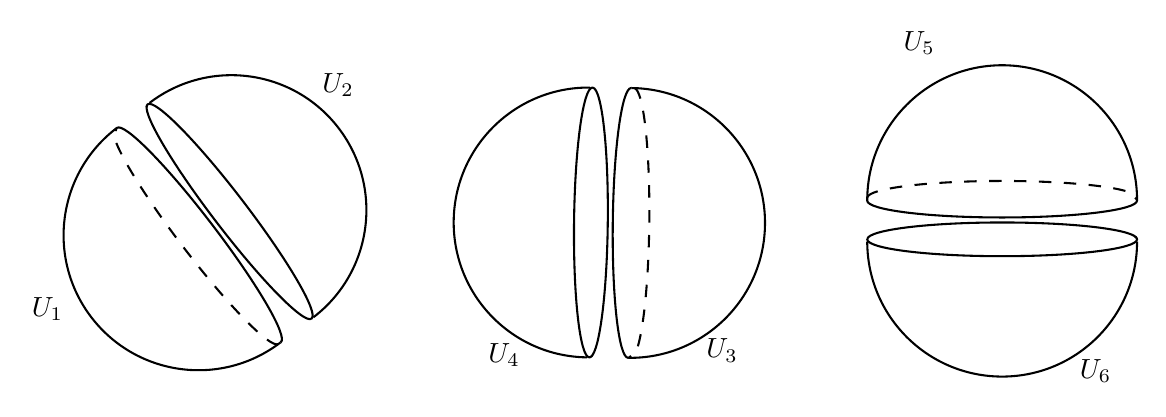
\begin{tikzpicture}[x=0.75pt,y=0.75pt,yscale=-1,xscale=1]
		%uncomment if require: \path (0,300); %set diagram left start at 0, and has height of 300
		
		%Shape: Arc [id:dp8087392079745468] 
		\draw  [draw opacity=0] (610,205) .. controls (610,205) and (610,205) .. (610,205) .. controls (610,240.9) and (580.9,270) .. (545,270) .. controls (509.1,270) and (480,240.9) .. (480,205) -- (545,205) -- cycle ; \draw   (610,205) .. controls (610,205) and (610,205) .. (610,205) .. controls (610,240.9) and (580.9,270) .. (545,270) .. controls (509.1,270) and (480,240.9) .. (480,205) ;  
		%Shape: Arc [id:dp7144643582066421] 
		\draw  [draw opacity=0] (480.02,203.67) .. controls (480.89,199.28) and (509.65,195.75) .. (545,195.75) .. controls (578.58,195.75) and (606.22,198.93) .. (609.64,203.02) -- (545,203.88) -- cycle ; \draw   (480.02,203.67) .. controls (480.89,199.28) and (509.65,195.75) .. (545,195.75) .. controls (578.58,195.75) and (606.22,198.93) .. (609.64,203.02) ;  
		%Shape: Arc [id:dp9774877190814104] 
		\draw  [draw opacity=0] (480,185) .. controls (480,185) and (480,185) .. (480,185) .. controls (480,149.1) and (509.1,120) .. (545,120) .. controls (580.9,120) and (610,149.1) .. (610,185) -- (545,185) -- cycle ; \draw   (480,185) .. controls (480,185) and (480,185) .. (480,185) .. controls (480,149.1) and (509.1,120) .. (545,120) .. controls (580.9,120) and (610,149.1) .. (610,185) ;  
		%Shape: Arc [id:dp7118645098131682] 
		\draw  [draw opacity=0] (609.09,202.51) .. controls (609.69,202.95) and (610,203.41) .. (610,203.88) .. controls (610,208.36) and (580.9,212) .. (545,212) .. controls (509.1,212) and (480,208.36) .. (480,203.88) .. controls (480,203.8) and (480.01,203.73) .. (480.02,203.66) -- (545,203.88) -- cycle ; \draw   (609.09,202.51) .. controls (609.69,202.95) and (610,203.41) .. (610,203.88) .. controls (610,208.36) and (580.9,212) .. (545,212) .. controls (509.1,212) and (480,208.36) .. (480,203.88) .. controls (480,203.8) and (480.01,203.73) .. (480.02,203.66) ;  
		%Shape: Arc [id:dp7962209595423704] 
		\draw  [draw opacity=0] (609.06,183.85) .. controls (609.66,184.29) and (609.98,184.75) .. (609.98,185.22) .. controls (609.98,189.7) and (580.88,193.34) .. (544.98,193.34) .. controls (509.08,193.34) and (479.98,189.7) .. (479.98,185.22) .. controls (479.98,185.14) and (479.99,185.07) .. (480,185) -- (544.98,185.22) -- cycle ; \draw   (609.06,183.85) .. controls (609.66,184.29) and (609.98,184.75) .. (609.98,185.22) .. controls (609.98,189.7) and (580.88,193.34) .. (544.98,193.34) .. controls (509.08,193.34) and (479.98,189.7) .. (479.98,185.22) .. controls (479.98,185.14) and (479.99,185.07) .. (480,185) ;  
		%Shape: Arc [id:dp26854896682720364] 
		\draw  [draw opacity=0][dash pattern={on 4.5pt off 4.5pt}] (480.02,183.67) .. controls (480.89,179.28) and (509.65,175.75) .. (545,175.75) .. controls (578.58,175.75) and (606.22,178.93) .. (609.64,183.02) -- (545,183.88) -- cycle ; \draw  [dash pattern={on 4.5pt off 4.5pt}] (480.02,183.67) .. controls (480.89,179.28) and (509.65,175.75) .. (545,175.75) .. controls (578.58,175.75) and (606.22,178.93) .. (609.64,183.02) ;  
		%Shape: Arc [id:dp8593027572319052] 
		\draw  [draw opacity=0] (345,260.74) .. controls (345,260.74) and (345,260.74) .. (345,260.74) .. controls (345,260.74) and (345,260.74) .. (345,260.74) .. controls (309.1,260.33) and (280.34,230.89) .. (280.75,195) .. controls (281.16,159.1) and (310.6,130.34) .. (346.49,130.75) -- (345.74,195.74) -- cycle ; \draw   (345,260.74) .. controls (345,260.74) and (345,260.74) .. (345,260.74) .. controls (345,260.74) and (345,260.74) .. (345,260.74) .. controls (309.1,260.33) and (280.34,230.89) .. (280.75,195) .. controls (281.16,159.1) and (310.6,130.34) .. (346.49,130.75) ;  
		%Shape: Arc [id:dp5017110012711772] 
		\draw  [draw opacity=0] (347.82,130.78) .. controls (352.2,131.7) and (355.4,160.5) .. (354.99,195.85) .. controls (354.61,229.43) and (351.11,257.03) .. (346.98,260.41) -- (346.87,195.76) -- cycle ; \draw   (347.82,130.78) .. controls (352.2,131.7) and (355.4,160.5) .. (354.99,195.85) .. controls (354.61,229.43) and (351.11,257.03) .. (346.98,260.41) ;  
		%Shape: Arc [id:dp34022749055732393] 
		\draw  [draw opacity=0] (366.49,130.98) .. controls (366.49,130.98) and (366.49,130.98) .. (366.49,130.98) .. controls (402.39,131.39) and (431.15,160.83) .. (430.74,196.72) .. controls (430.33,232.62) and (400.89,261.38) .. (364.99,260.97) -- (365.74,195.97) -- cycle ; \draw   (366.49,130.98) .. controls (366.49,130.98) and (366.49,130.98) .. (366.49,130.98) .. controls (402.39,131.39) and (431.15,160.83) .. (430.74,196.72) .. controls (430.33,232.62) and (400.89,261.38) .. (364.99,260.97) ;  
		%Shape: Arc [id:dp9156415467589833] 
		\draw  [draw opacity=0] (347.5,259.86) .. controls (347.05,260.45) and (346.59,260.76) .. (346.12,260.75) .. controls (341.63,260.7) and (338.33,231.56) .. (338.74,195.66) .. controls (339.16,159.77) and (343.13,130.71) .. (347.62,130.76) .. controls (347.69,130.76) and (347.76,130.77) .. (347.83,130.79) -- (346.87,195.76) -- cycle ; \draw   (347.5,259.86) .. controls (347.05,260.45) and (346.59,260.76) .. (346.12,260.75) .. controls (341.63,260.7) and (338.33,231.56) .. (338.74,195.66) .. controls (339.16,159.77) and (343.13,130.71) .. (347.62,130.76) .. controls (347.69,130.76) and (347.76,130.77) .. (347.83,130.79) ;  
		%Shape: Arc [id:dp7534866185784517] 
		\draw  [draw opacity=0] (366.15,260.05) .. controls (365.7,260.64) and (365.24,260.95) .. (364.78,260.95) .. controls (360.29,260.89) and (356.99,231.75) .. (357.4,195.86) .. controls (357.82,159.96) and (361.79,130.9) .. (366.28,130.95) .. controls (366.35,130.96) and (366.42,130.96) .. (366.49,130.98) -- (365.53,195.95) -- cycle ; \draw   (366.15,260.05) .. controls (365.7,260.64) and (365.24,260.95) .. (364.78,260.95) .. controls (360.29,260.89) and (356.99,231.75) .. (357.4,195.86) .. controls (357.82,159.96) and (361.79,130.9) .. (366.28,130.95) .. controls (366.35,130.96) and (366.42,130.96) .. (366.49,130.98) ;  
		%Shape: Arc [id:dp7058755896129407] 
		\draw  [draw opacity=0][dash pattern={on 4.5pt off 4.5pt}] (367.82,131.01) .. controls (372.2,131.93) and (375.4,160.73) .. (374.99,196.08) .. controls (374.61,229.66) and (371.1,257.26) .. (366.98,260.64) -- (366.87,195.99) -- cycle ; \draw  [dash pattern={on 4.5pt off 4.5pt}] (367.82,131.01) .. controls (372.2,131.93) and (375.4,160.73) .. (374.99,196.08) .. controls (374.61,229.66) and (371.1,257.26) .. (366.98,260.64) ;  
		%Shape: Arc [id:dp6580687340920708] 
		\draw  [draw opacity=0] (134.21,138.15) .. controls (134.21,138.15) and (134.21,138.15) .. (134.21,138.15) .. controls (134.21,138.15) and (134.21,138.15) .. (134.21,138.15) .. controls (162.73,116.35) and (203.52,121.79) .. (225.32,150.31) .. controls (247.13,178.82) and (241.69,219.62) .. (213.17,241.42) -- (173.69,189.79) -- cycle ; \draw   (134.21,138.15) .. controls (134.21,138.15) and (134.21,138.15) .. (134.21,138.15) .. controls (134.21,138.15) and (134.21,138.15) .. (134.21,138.15) .. controls (162.73,116.35) and (203.52,121.79) .. (225.32,150.31) .. controls (247.13,178.82) and (241.69,219.62) .. (213.17,241.42) ;  
		%Shape: Arc [id:dp04807301977746614] 
		\draw  [draw opacity=0] (212.1,242.21) .. controls (208.08,244.19) and (187.81,223.49) .. (166.34,195.4) .. controls (145.94,168.73) and (131.69,144.84) .. (132.85,139.64) -- (172.79,190.47) -- cycle ; \draw   (212.1,242.21) .. controls (208.08,244.19) and (187.81,223.49) .. (166.34,195.4) .. controls (145.94,168.73) and (131.69,144.84) .. (132.85,139.64) ;  
		%Shape: Arc [id:dp5373023961242778] 
		\draw  [draw opacity=0] (197.28,253.57) .. controls (197.28,253.57) and (197.28,253.57) .. (197.28,253.57) .. controls (197.28,253.57) and (197.28,253.57) .. (197.28,253.57) .. controls (168.76,275.37) and (127.97,269.93) .. (106.16,241.41) .. controls (84.36,212.89) and (89.8,172.1) .. (118.32,150.3) -- (157.8,201.93) -- cycle ; \draw   (197.28,253.57) .. controls (197.28,253.57) and (197.28,253.57) .. (197.28,253.57) .. controls (197.28,253.57) and (197.28,253.57) .. (197.28,253.57) .. controls (168.76,275.37) and (127.97,269.93) .. (106.16,241.41) .. controls (84.36,212.89) and (89.8,172.1) .. (118.32,150.3) ;  
		%Shape: Arc [id:dp6075301311311689] 
		\draw  [draw opacity=0] (132.79,140.39) .. controls (132.77,139.64) and (132.95,139.11) .. (133.31,138.83) .. controls (136.88,136.11) and (157.44,157.02) .. (179.25,185.53) .. controls (201.05,214.05) and (215.84,239.38) .. (212.27,242.11) .. controls (212.22,242.15) and (212.15,242.19) .. (212.09,242.22) -- (172.79,190.47) -- cycle ; \draw   (132.79,140.39) .. controls (132.77,139.64) and (132.95,139.11) .. (133.31,138.83) .. controls (136.88,136.11) and (157.44,157.02) .. (179.25,185.53) .. controls (201.05,214.05) and (215.84,239.38) .. (212.27,242.11) .. controls (212.22,242.15) and (212.15,242.19) .. (212.09,242.22) ;  
		%Shape: Arc [id:dp4893987696896971] 
		\draw  [draw opacity=0] (117.98,151.74) .. controls (117.96,150.99) and (118.14,150.47) .. (118.5,150.18) .. controls (122.07,147.46) and (142.64,168.37) .. (164.44,196.89) .. controls (186.24,225.4) and (201.03,250.73) .. (197.46,253.46) .. controls (197.41,253.5) and (197.34,253.54) .. (197.28,253.57) -- (157.98,201.82) -- cycle ; \draw   (117.98,151.74) .. controls (117.96,150.99) and (118.14,150.47) .. (118.5,150.18) .. controls (122.07,147.46) and (142.64,168.37) .. (164.44,196.89) .. controls (186.24,225.4) and (201.03,250.73) .. (197.46,253.46) .. controls (197.41,253.5) and (197.34,253.54) .. (197.28,253.57) ;  
		%Shape: Arc [id:dp5010740042347757] 
		\draw  [draw opacity=0][dash pattern={on 4.5pt off 4.5pt}] (196.21,254.36) .. controls (192.19,256.34) and (171.92,235.64) .. (150.45,207.55) .. controls (130.05,180.87) and (115.8,156.99) .. (116.96,151.78) -- (156.91,202.62) -- cycle ; \draw  [dash pattern={on 4.5pt off 4.5pt}] (196.21,254.36) .. controls (192.19,256.34) and (171.92,235.64) .. (150.45,207.55) .. controls (130.05,180.87) and (115.8,156.99) .. (116.96,151.78) ;  
		
		% Text Node
		\draw (76,230.4) node [anchor=north west][inner sep=0.75pt]    {$U_{1}$};
		% Text Node
		\draw (216,122.4) node [anchor=north west][inner sep=0.75pt]    {$U_{2}$};
		% Text Node
		\draw (401,250.4) node [anchor=north west][inner sep=0.75pt]    {$U_{3}$};
		% Text Node
		\draw (296,252.4) node [anchor=north west][inner sep=0.75pt]    {$U_{4}$};
		% Text Node
		\draw (496,102.4) node [anchor=north west][inner sep=0.75pt]    {$U_{5}$};
		% Text Node
		\draw (581,260.4) node [anchor=north west][inner sep=0.75pt]    {$U_{6}$};
		
		
	\end{tikzpicture}
\end{figure}
\end{problem}
\begin{solution}
	For the set $ U_1 \cap U_4 $ we have
	\[ U_1 \cap U_4 = \set{(x,y,z) \in S^2\ :\ x>0 \text{ and } y < 0 }. \]
	Thus we will have
	\[ \phi_4(U_1\cap U_4) = \set{(x,z)\in \R^2 \ :\ x^2 + z^2 \leq 1,\ x>0}. \]
	Thus we can write
	\[ (\phi_1 \circ \inv{\phi_4})(\langle x,z \rangle ) = \phi_1(\langle x,-\sqrt{1-(x^2+y^2)},z \rangle) = \langle -\sqrt{1-(x^2+y^2)},z \rangle  \]
	This is indeed a $ C^\infty $ vector valued function, since each component is a $ C^\infty $ function. Now to evaluate $ \phi_4 \circ \inv{\phi_1}: \phi_1(U_1 \cap U_4) \to \phi_4(U_1\cap U_4) $ we need to first evaluate the set $ \phi_1(U_1 \cap U_4) $. For this set we have
	\[ \phi_1(U_1 \cap U_4) = \set{(z,y)\in\R^2\ :\ z^2 + y^2 \leq 1, y < 0}. \]
	Then we can write
	\[ (\phi_4 \circ \inv{\phi_1})(\langle y,z \rangle ) = \phi_4(\langle \sqrt{1-(y^2+z^2)}, y,z  \rangle) = \langle \sqrt{1-(y^2+z^2)} , z \rangle. \]
	This is indeed a $ C^\infty $ vector valued function. 
	
	To evaluate the function $ \phi_6 \circ \inv{\phi}_1: \phi_1(U_1 \cap U_6) \to \phi_6(U_1 \cap U_6) $, we first need to determine the domain of this function. First observe that 
	\[ U_1 \cap U_6 =  \set{(x,y,z) \in S^2\ :\ x>0 \text{ and } y<0}, \]
	which is the same as $ U_1 \cap U_4 $. Then for the domain of the function of interest we can write
	\[ \phi_1(U_1 \cap U_6) = \set{(y,z) \in \R^2 :\ z^2 + y^2 \leq 1 \text{ and } y<0}, \]
	\[ (\phi_6 \circ \inv{\phi_1})(\langle y,z \rangle) = \phi_6(\langle \sqrt{1-(y^2+z^2)},y,z \rangle) = \langle \sqrt{1-(y^2+z^2)}, y \rangle. \]
\end{solution}

\begin{problem}[Existence of a coordinate neighborhood (from W. Tu)]
	Let $ \set{(U_\alpha, \phi_\alpha)}_{\alpha \in I} $ be the maximal atlas on manifold $ M $. For any open set $ U $ in $ M $ and a point $ p \in U $, prove the existence of a coordinate open set $ U_\alpha $ such that $ p \in U_\alpha \subset U $.
\end{problem}
\begin{solution}
	Since $ \set{(U_\alpha,\phi_\alpha)}_{\alpha \in I} $ is an atlas, then for $ p \in U $ given as above, we can find some $ \alpha_1 \in I $ such that $ p \in U_{\alpha_1} $. Consider the open set $ W = U_{\alpha_1} \cap U $. The chart $ (W, \phi_{\alpha_1}|_W) $ is in the atlas (since it is maximal), i.e. $ \exists \alpha \in I $ such that $ (U_\alpha, \phi_\alpha) = (W, \phi_{\alpha_1}|_W) $. This completes the proof.
\end{solution}

\begin{problem}[An atlas for a product manifold (from W. Tu)]
	Prove the following proposition.
	\begin{proposition}
		If $ \set{(U_\alpha,\phi_\alpha)} $ and $ \set{(V_i,\psi_i)} $ are $ C^\infty $ atlases for the manifold $ M $ and $ N $ of dimensions $ m $ and $ n $, respectively, then the collection 
		\[ \set{(U_\alpha \times V_i,\phi_\alpha \times \psi_i)} \] where
		\[ \phi_\alpha \times \psi_i\ :\ U_\alpha \times V_i \to \R^m \times \R^n \]
		of charts is a $ C^\infty $ atlas on $ M\times N $. Therefore, $ M\times N $ is a $ C^\infty $ manifold of dimension $ m+n $.
	\end{proposition}
\end{problem}
\begin{solution}
	In order to show that the collection $ \frak{U} = \set{(U_\alpha \times V_i, \phi_\alpha \times \psi_i)} $ is an atlas for $ M\times N $, we need to show that charts are pairwise compatible as well as the set covering the whole space. To show that the chart covers the whole space $ M\times N $, let $ (p_1,p_2) \in M\times N $. Then $ p_1 \in M $ and $ p_2 \in N $. Then there are two coordinate open sets such that $ p_1 \in U_{\alpha_1} $ and $ p_2 \in V_{i_1} $. Thus the coordinate open set $ U_{\alpha_1} \times V_{i_1} $ contains the point $ (p_1,p_2) $.
	
	To show that two any two charts in the collection $ \frak{U} $ are compatible, let $ (U_{\alpha_1} \times V_{i_1},\phi_{\alpha_1}\times \psi_{i_1}) $ and $  (U_{\alpha_2} \times V_{i_2},\phi_{\alpha_2}\times \psi_{i_2}) $ be two  charts. We claim that the corresponding coordinate maps are $ C^\infty $. This follows directly from the fact the each component of the map these coordinate maps are $ C^\infty $.
\end{solution}

\begin{problem}[Smoothness of a projection map (from W. Tu)]
	Let $ M $ and $ N $ be manifolds and $ \pi: M\times N \to M $, $ \pi(p,q) = p $ the projection to the first factor. Prove that $ \pi $ is a $ C^\infty $ map.
\end{problem}

\begin{solution}
	Let $ p \in M $ and $ q \in N $, thus $ (p,q) \in M\times N $. Let $ \phi $ and $ \psi $ be two coordinate maps such that $ \phi(p) = x $ and $ \psi(q) = y $. Thus we can write $ (\phi, \psi)(p,q) = (x,y) $. Consider the function
	\[ (\phi \circ \pi \circ (\phi\times \psi)^{-1})(x,y) = \phi(\pi(p,q)) = \phi(p) = x.  \]
	The function above is a $ \C^\infty $ map from $ \R^{n+m} $ to $ \R^n $ (assuming $ M, N $ are $ m $ and $ n $ dimensional manifolds). This proves that the projection map $ \pi $ is smooth.
\end{solution}

\begin{problem}[Smoothness of a map tp a Cartesian product (from W. Tu)]
	Let $ M_1, M_2 $, and $ N $ be manifolds of dimensions $ m_1,m_2 $ and $ n $ respectively. Prove that a map $ (f_1,f_2): N \to M_1\times M_2 $ is smooth if and only if $ f_i:N\to M $ for $ i=1,2 $ are both smooth.
\end{problem} 

\begin{solution}
	Consider the following picture.
	\begin{figure}[h!]
	\centering
	
	
	
	
	\tikzset{every picture/.style={line width=0.75pt}} %set default line width to 0.75pt        
	
	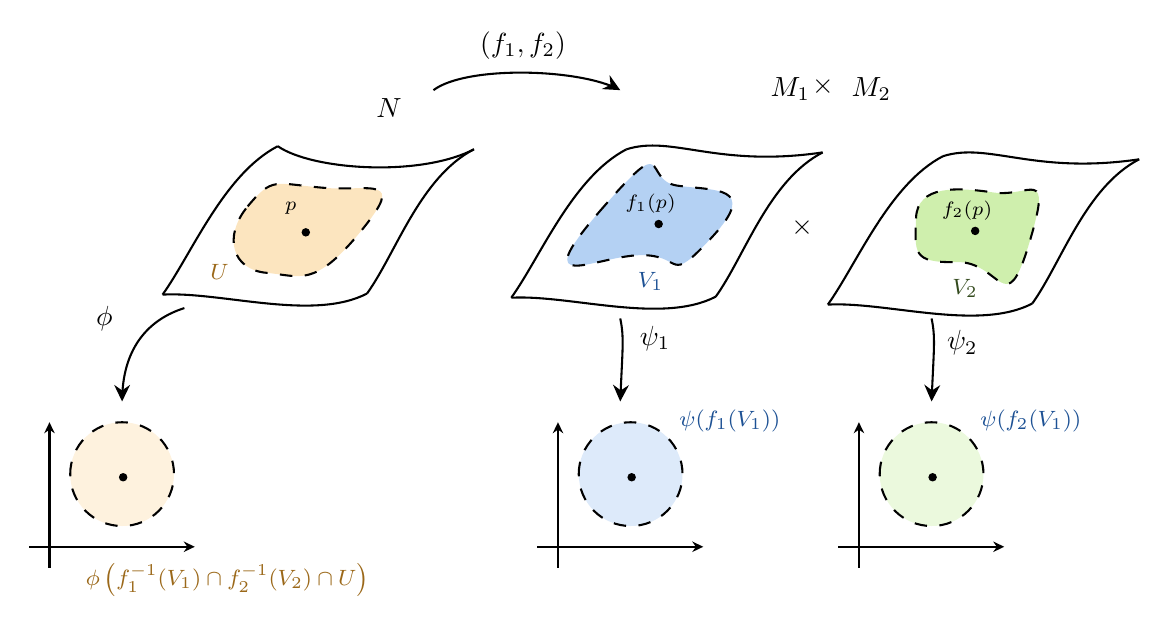
\begin{tikzpicture}[x=0.75pt,y=0.75pt,yscale=-1,xscale=1]
		%uncomment if require: \path (0,300); %set diagram left start at 0, and has height of 300
		
		%Curve Lines [id:da10777202147976128] 
		\draw    (89.5,138.5) .. controls (103.5,119) and (119,80.5) .. (145,67) ;
		%Curve Lines [id:da9226409814736687] 
		\draw    (89.5,138.5) .. controls (118,137) and (162,151.5) .. (188,138) ;
		%Curve Lines [id:da6153501766442295] 
		\draw    (188,138) .. controls (202,118.5) and (213.5,82) .. (239.5,68.5) ;
		%Curve Lines [id:da8299437341096081] 
		\draw    (145,67) .. controls (161.5,78.5) and (213.5,82) .. (239.5,68.5) ;
		%Curve Lines [id:da708998797665932] 
		\draw    (257.5,140) .. controls (271.5,120.5) and (287,82) .. (313,68.5) ;
		%Curve Lines [id:da5763078865113123] 
		\draw    (257.5,140) .. controls (286,138.5) and (330,153) .. (356,139.5) ;
		%Curve Lines [id:da17448723811544053] 
		\draw    (356,139.5) .. controls (370,120) and (381.5,83.5) .. (407.5,70) ;
		%Curve Lines [id:da5843329628503129] 
		\draw    (313,68.5) .. controls (335,61.5) and (356.5,77.5) .. (407.5,70) ;
		%Shape: Polygon Curved [id:ds719249129813768] 
		\draw  [fill={rgb, 255:red, 245; green, 166; blue, 35 }  ,fill opacity=0.29 ][dash pattern={on 4.5pt off 4.5pt}] (130.5,96) .. controls (142.5,81.5) and (143.5,85) .. (166.5,87) .. controls (189.5,89) and (207.5,80.5) .. (185,108) .. controls (162.5,135.5) and (156,129.5) .. (139.5,128) .. controls (123,126.5) and (118.5,110.5) .. (130.5,96) -- cycle ;
		%Shape: Polygon Curved [id:ds20297397591709365] 
		\draw  [fill={rgb, 255:red, 74; green, 144; blue, 226 }  ,fill opacity=0.41 ][dash pattern={on 4.5pt off 4.5pt}] (300,98.5) .. controls (335.5,57.5) and (320,83.5) .. (337.5,86) .. controls (355,88.5) and (377,86) .. (354.5,110.5) .. controls (332,135) and (341,119) .. (319.5,119.5) .. controls (298,120) and (264.5,139.5) .. (300,98.5) -- cycle ;
		%Straight Lines [id:da8177031700071737] 
		\draw    (35,203) -- (35,270) ;
		\draw [shift={(35,200)}, rotate = 90] [fill={rgb, 255:red, 0; green, 0; blue, 0 }  ][line width=0.08]  [draw opacity=0] (5.36,-2.57) -- (0,0) -- (5.36,2.57) -- (3.56,0) -- cycle    ;
		%Straight Lines [id:da5847590524068735] 
		\draw    (102,260) -- (25,260) ;
		\draw [shift={(105,260)}, rotate = 180] [fill={rgb, 255:red, 0; green, 0; blue, 0 }  ][line width=0.08]  [draw opacity=0] (5.36,-2.57) -- (0,0) -- (5.36,2.57) -- (3.56,0) -- cycle    ;
		%Shape: Circle [id:dp5757945587417739] 
		\draw  [fill={rgb, 255:red, 245; green, 166; blue, 35 }  ,fill opacity=0.15 ][dash pattern={on 4.5pt off 4.5pt}] (45,225) .. controls (45,211.19) and (56.19,200) .. (70,200) .. controls (83.81,200) and (95,211.19) .. (95,225) .. controls (95,238.81) and (83.81,250) .. (70,250) .. controls (56.19,250) and (45,238.81) .. (45,225) -- cycle ;
		%Straight Lines [id:da9243110317223102] 
		\draw    (280,203) -- (280,270) ;
		\draw [shift={(280,200)}, rotate = 90] [fill={rgb, 255:red, 0; green, 0; blue, 0 }  ][line width=0.08]  [draw opacity=0] (5.36,-2.57) -- (0,0) -- (5.36,2.57) -- (3.56,0) -- cycle    ;
		%Straight Lines [id:da35917271861832445] 
		\draw    (347,260) -- (270,260) ;
		\draw [shift={(350,260)}, rotate = 180] [fill={rgb, 255:red, 0; green, 0; blue, 0 }  ][line width=0.08]  [draw opacity=0] (5.36,-2.57) -- (0,0) -- (5.36,2.57) -- (3.56,0) -- cycle    ;
		%Shape: Circle [id:dp7567118959752777] 
		\draw  [fill={rgb, 255:red, 74; green, 144; blue, 226 }  ,fill opacity=0.19 ][dash pattern={on 4.5pt off 4.5pt}] (290,225) .. controls (290,211.19) and (301.19,200) .. (315,200) .. controls (328.81,200) and (340,211.19) .. (340,225) .. controls (340,238.81) and (328.81,250) .. (315,250) .. controls (301.19,250) and (290,238.81) .. (290,225) -- cycle ;
		%Curve Lines [id:da8387568355499948] 
		\draw    (220,40) .. controls (235.36,28.48) and (286.66,29.4) .. (307.55,38.78) ;
		\draw [shift={(310,40)}, rotate = 208.93] [fill={rgb, 255:red, 0; green, 0; blue, 0 }  ][line width=0.08]  [draw opacity=0] (8.04,-3.86) -- (0,0) -- (8.04,3.86) -- (5.34,0) -- cycle    ;
		%Curve Lines [id:da5596780294001671] 
		\draw    (310,150) .. controls (311.92,159.12) and (311.08,164.55) .. (310.12,187.09) ;
		\draw [shift={(310,190)}, rotate = 272.29] [fill={rgb, 255:red, 0; green, 0; blue, 0 }  ][line width=0.08]  [draw opacity=0] (8.04,-3.86) -- (0,0) -- (8.04,3.86) -- (5.34,0) -- cycle    ;
		%Curve Lines [id:da33319736118491083] 
		\draw    (100,145) .. controls (83.11,150.31) and (70.88,163.53) .. (70.05,187.36) ;
		\draw [shift={(70,190)}, rotate = 270] [fill={rgb, 255:red, 0; green, 0; blue, 0 }  ][line width=0.08]  [draw opacity=0] (8.04,-3.86) -- (0,0) -- (8.04,3.86) -- (5.34,0) -- cycle    ;
		%Shape: Circle [id:dp912491598557873] 
		\draw  [fill={rgb, 255:red, 0; green, 0; blue, 0 }  ,fill opacity=1 ] (157,108.5) .. controls (157,107.67) and (157.67,107) .. (158.5,107) .. controls (159.33,107) and (160,107.67) .. (160,108.5) .. controls (160,109.33) and (159.33,110) .. (158.5,110) .. controls (157.67,110) and (157,109.33) .. (157,108.5) -- cycle ;
		%Shape: Circle [id:dp5874182665613439] 
		\draw  [fill={rgb, 255:red, 0; green, 0; blue, 0 }  ,fill opacity=1 ] (327,104.5) .. controls (327,103.67) and (327.67,103) .. (328.5,103) .. controls (329.33,103) and (330,103.67) .. (330,104.5) .. controls (330,105.33) and (329.33,106) .. (328.5,106) .. controls (327.67,106) and (327,105.33) .. (327,104.5) -- cycle ;
		%Shape: Circle [id:dp6918787727605586] 
		\draw  [fill={rgb, 255:red, 0; green, 0; blue, 0 }  ,fill opacity=1 ] (69,226.5) .. controls (69,225.67) and (69.67,225) .. (70.5,225) .. controls (71.33,225) and (72,225.67) .. (72,226.5) .. controls (72,227.33) and (71.33,228) .. (70.5,228) .. controls (69.67,228) and (69,227.33) .. (69,226.5) -- cycle ;
		%Shape: Circle [id:dp5802827719353891] 
		\draw  [fill={rgb, 255:red, 0; green, 0; blue, 0 }  ,fill opacity=1 ] (314,226.5) .. controls (314,225.67) and (314.67,225) .. (315.5,225) .. controls (316.33,225) and (317,225.67) .. (317,226.5) .. controls (317,227.33) and (316.33,228) .. (315.5,228) .. controls (314.67,228) and (314,227.33) .. (314,226.5) -- cycle ;
		%Curve Lines [id:da5866172687533027] 
		\draw    (410,143.32) .. controls (424,123.82) and (439.5,85.32) .. (465.5,71.82) ;
		%Curve Lines [id:da33769380232352386] 
		\draw    (410,143.32) .. controls (438.5,141.82) and (482.5,156.32) .. (508.5,142.82) ;
		%Curve Lines [id:da5667601010223242] 
		\draw    (508.5,142.82) .. controls (522.5,123.32) and (534,86.82) .. (560,73.32) ;
		%Curve Lines [id:da7766245611502776] 
		\draw    (465.5,71.82) .. controls (487.5,64.82) and (509,80.82) .. (560,73.32) ;
		%Shape: Polygon Curved [id:ds9848033990053162] 
		\draw  [fill={rgb, 255:red, 126; green, 211; blue, 33 }  ,fill opacity=0.37 ][dash pattern={on 4.5pt off 4.5pt}] (452.5,101.82) .. controls (453,85.5) and (472.5,86.82) .. (490,89.32) .. controls (507.5,91.82) and (518.5,75.5) .. (507,113.82) .. controls (495.5,152.14) and (493.5,122.32) .. (472,122.82) .. controls (450.5,123.32) and (452,118.14) .. (452.5,101.82) -- cycle ;
		%Shape: Circle [id:dp8441479070293367] 
		\draw  [fill={rgb, 255:red, 0; green, 0; blue, 0 }  ,fill opacity=1 ] (479.5,107.82) .. controls (479.5,106.99) and (480.17,106.32) .. (481,106.32) .. controls (481.83,106.32) and (482.5,106.99) .. (482.5,107.82) .. controls (482.5,108.65) and (481.83,109.32) .. (481,109.32) .. controls (480.17,109.32) and (479.5,108.65) .. (479.5,107.82) -- cycle ;
		%Straight Lines [id:da4245600664130684] 
		\draw    (425,203) -- (425,270) ;
		\draw [shift={(425,200)}, rotate = 90] [fill={rgb, 255:red, 0; green, 0; blue, 0 }  ][line width=0.08]  [draw opacity=0] (5.36,-2.57) -- (0,0) -- (5.36,2.57) -- (3.56,0) -- cycle    ;
		%Straight Lines [id:da8383634096867163] 
		\draw    (492,260) -- (415,260) ;
		\draw [shift={(495,260)}, rotate = 180] [fill={rgb, 255:red, 0; green, 0; blue, 0 }  ][line width=0.08]  [draw opacity=0] (5.36,-2.57) -- (0,0) -- (5.36,2.57) -- (3.56,0) -- cycle    ;
		%Shape: Circle [id:dp032856070596776865] 
		\draw  [fill={rgb, 255:red, 184; green, 233; blue, 134 }  ,fill opacity=0.28 ][dash pattern={on 4.5pt off 4.5pt}] (435,225) .. controls (435,211.19) and (446.19,200) .. (460,200) .. controls (473.81,200) and (485,211.19) .. (485,225) .. controls (485,238.81) and (473.81,250) .. (460,250) .. controls (446.19,250) and (435,238.81) .. (435,225) -- cycle ;
		%Shape: Circle [id:dp2655157582176253] 
		\draw  [fill={rgb, 255:red, 0; green, 0; blue, 0 }  ,fill opacity=1 ] (459,226.5) .. controls (459,225.67) and (459.67,225) .. (460.5,225) .. controls (461.33,225) and (462,225.67) .. (462,226.5) .. controls (462,227.33) and (461.33,228) .. (460.5,228) .. controls (459.67,228) and (459,227.33) .. (459,226.5) -- cycle ;
		%Curve Lines [id:da36500972985566005] 
		\draw    (460,150) .. controls (461.92,159.12) and (461.08,164.55) .. (460.12,187.09) ;
		\draw [shift={(460,190)}, rotate = 272.29] [fill={rgb, 255:red, 0; green, 0; blue, 0 }  ][line width=0.08]  [draw opacity=0] (8.04,-3.86) -- (0,0) -- (8.04,3.86) -- (5.34,0) -- cycle    ;
		
		% Text Node
		\draw (191,42.4) node [anchor=north west][inner sep=0.75pt]    {$N$};
		% Text Node
		\draw (381,32.4) node [anchor=north west][inner sep=0.75pt]    {$M_{1}$};
		% Text Node
		\draw (241,10.4) node [anchor=north west][inner sep=0.75pt]    {$( f_{1} ,f_{2})$};
		% Text Node
		\draw (318,152.4) node [anchor=north west][inner sep=0.75pt]    {$\psi _{1}$};
		% Text Node
		\draw (56,142.4) node [anchor=north west][inner sep=0.75pt]    {$\phi $};
		% Text Node
		\draw (147,92.4) node [anchor=north west][inner sep=0.75pt]  [font=\scriptsize]  {$p$};
		% Text Node
		\draw (311,88.4) node [anchor=north west][inner sep=0.75pt]  [font=\scriptsize]  {$f_{1}( p)$};
		% Text Node
		\draw (111,122.4) node [anchor=north west][inner sep=0.75pt]  [font=\footnotesize,color={rgb, 255:red, 155; green, 104; blue, 25 }  ,opacity=1 ]  {$U$};
		% Text Node
		\draw (317,126.4) node [anchor=north west][inner sep=0.75pt]  [font=\footnotesize,color={rgb, 255:red, 29; green, 81; blue, 148 }  ,opacity=1 ]  {$V_{1}$};
		% Text Node
		\draw (337,192.4) node [anchor=north west][inner sep=0.75pt]  [font=\footnotesize,color={rgb, 255:red, 29; green, 81; blue, 148 }  ,opacity=1 ]  {$\psi ( f_{1}( V_{1}))$};
		% Text Node
		\draw (51,266.4) node [anchor=north west][inner sep=0.75pt]  [font=\footnotesize,color={rgb, 255:red, 155; green, 104; blue, 25 }  ,opacity=1 ]  {$\phi \left( f_{1}^{-1}( V_{1}) \cap f_{2}^{-1}( V_{2}) \cap U\right)$};
		% Text Node
		\draw (463.5,91.72) node [anchor=north west][inner sep=0.75pt]  [font=\scriptsize]  {$f_{2}( p)$};
		% Text Node
		\draw (468.5,129.72) node [anchor=north west][inner sep=0.75pt]  [font=\footnotesize,color={rgb, 255:red, 52; green, 75; blue, 30 }  ,opacity=1 ]  {$V_{2}$};
		% Text Node
		\draw (482,192.4) node [anchor=north west][inner sep=0.75pt]  [font=\footnotesize,color={rgb, 255:red, 29; green, 81; blue, 148 }  ,opacity=1 ]  {$\psi ( f_{2}( V_{1}))$};
		% Text Node
		\draw (420,32.4) node [anchor=north west][inner sep=0.75pt]    {$M_{2}$};
		% Text Node
		\draw (391,100.4) node [anchor=north west][inner sep=0.75pt]    {$\times $};
		% Text Node
		\draw (466,154.4) node [anchor=north west][inner sep=0.75pt]    {$\psi _{2}$};
		% Text Node
		\draw (401,32.4) node [anchor=north west][inner sep=0.75pt]    {$\times $};
		
		
	\end{tikzpicture}
\end{figure}
	\FloatBarrier
	
	For the first direction, we will show that smoothness of $ (f_1,f_2): N \to M_1\times M_2 $ implies the smoothness of $ f_1:N\to M_1 $ and $ f_2: N \to M_2 $. As depicted in the picture above, let $ \phi $ be a coordinate map for $ N $ and $ \psi_1, \psi_2 $ be coordinate maps for $ M_1,M_2 $ respectively. Since $ (f_1,f_2) $ is smooth, then $ (\psi_1 \times \psi_2) \circ (f_1,f_2) $ is smooth. Let $ p \in N $, then
	\[ ((\psi_1 \times \psi_2) \circ (f_1,f_2) \circ \inv{\phi})(\phi(p)) =
	((\psi_1 \times \psi_2) \circ (f_1,f_2)) (p) = (\psi_1\times \psi_2)(f_1(p),f_2(p)) = (\psi_1(f_1(p)), \psi_2(f_2(p))).
	 \]
	This is a smooth map from $ \R^n $ to $ \R^{m_1+m_2} $. Thus the components of the function are also smooth.
	
	For the converse, we need to show that the smoothness of $ f_1 $ and $ f_2 $ implies the smoothness of $ (f_1,f_2) $. Similar to the argument above, the smoothness of $ (f_1,f_2) $ follows immediately from the smoothness of the components.
\end{solution}

\begin{problem}[Smooth functions on unit circle (W. Tu)]
	We have studied before that the unit circle $ S^1 $ defined by $ x^2 + y^2 = 1 $ in $ \R^2 $ is a $ C^\infty $ manifold. Prove that a smooth function $ f: \R^2 \to \R $ defined on $ \R^2 $ restricts to a $ C^\infty $ function on $ S^1 $.
\end{problem}

\begin{solution}
	Consider the following inclusion map
	\[ i: S^1 \to \R^2 \]
	defined as $ i(p) = (x(p),y(p)) $, where $ x,y $ are the standard coordinate functions. The restriction of $ f $ to manifold will be
	\[ f|_{S^1} = f \circ i. \]
	To show that $ f|_{S^1} $ is smooth, we just need to show that the inclusion map is smooth. To show this we need to show that the components of this vector valued function is smooth. We start by showing that $ x $ is smooth. We use the same charts as in \autoref{problem:S^1Charts}. Let $ p \in S^1 $. If $ p \in U_3 \cap U_4 $ then we have
	\[ \mathds{1}_{(0,1)}\circ x \circ \inv{\phi_3} = \mathds{1}_{(0,1)}: (-1,1) \to \R^2, \qquad \mathds{1}_{(0,1)}\circ x \circ \inv{\phi_4} = \mathds{1}_{(0,1)}: (-1,1) \to \R^2,  \]
	which are both identity maps, thus smooth. So $  x $ is smooth on $ U_3\cap U_4 $. For $ U_1 $ we have
	\[ \mathds{1}_{(0,1)}\circ x \circ \inv{\phi_1}(x) = -\sqrt{1-x^2}, \qquad\text{for } x \in \phi_1(U_1) = (-1,1) \]
	thus $ x $ is smooth on $ U_1 $ as well. For $ U_2 $ we have
	\[ \mathds{1}_{(0,1)}\circ x \circ \inv{\phi_2}(x) = \sqrt{1-x^2}, \qquad\text{for } x \in \phi_2(U_2) = (-1,1) \]
	thus $  x $ is smooth on $ U_2  $ as well. We can use a similar strategy to show that the coordinate function $ y $ is also smooth.
\end{solution}



\begin{problem}
	The general linear group $ \operatorname{GL}(n,\R) $ is the set of all real valued matrices with non-zero determinant under matrix multiplication. In other words
	\[ \operatorname{GL}(n,\R) = \set{A = \left[ a_{ij} \right] \in \R^{n\times n}\ |\ \det(A) \neq 0} . \]
	We can see this as an open subset of $ \R^{n\times n} $, thus it is a manifold. Show that this forms a Lie group.
\end{problem}

\begin{solution}
	Let $ A,B $ be two matrices in the manifold. Then the $ i,j $ element of $ AB $ is
	\[ (AB)_{ij} = \sum_{k=1}^{n} A_{ik}B_{kj} \]
	which is a polynomial in the coordinates of $ A $ and $ B $, thus it is smooth. To show that the inverse is also smooth, for any function $ A $ in the manifold we have
	\[ \inv{A} = \frac{1}{\det(A)} \cdot (-1)^{i+j}((i,j)\text{- minor of $ A $}). \]
	The $ (i,j)\text{-minor} $ of matrix $ A $ is the determinant of the sub matrix by deleting the $ i\text{-th} $ row and $ j\text{th} $ column, which is again a polynomial in the coordinates of $ A $ and $ B $, thus smooth (given that $ \det(A) \neq 0 $).
\end{solution}

\begin{problem}[Jacobian matrix os a transition map (form W. Tu)]
	Let $ (U,\phi) = (U,x^1,\cdots,x^n) $ and $ (V,\psi) = (V,y^1,\cdots,y^n) $ be overlapping charts on a manifold $ M $. The transition map $ \psi \circ\inv{\phi}: \phi(U\cap V) \to \psi(U\cap V) $ is a diffeomorphism of open subsets of $ \R^n $. Show that its Jacobian matrix $ J(\psi\circ\inv{\phi}) $ at $ \phi(p) $ is the matrix $ [\partial y^i/\partial x^j] $ of partial derivatives at $ p $.
\end{problem}
\begin{solution}
	From the definition of the Jacobian matrix we can write
	\[ J(\psi \circ \inv{\phi}) = \frac{\partial (\psi \circ \inv{\phi})^i}{\partial r^j} =  \frac{\partial (r^i \circ \psi \circ \inv{\phi})}{\partial r^j} = \frac{\partial (y^i \circ \inv{\phi})}{\partial r^j} = \frac{\partial y^i}{\partial x^j}. \]
\end{solution}

\begin{observation}[Some mnemonics for the Jacobian matrix]
	Here I introduce a symbolic mnemonic of remembering the form of the Jacobian matrix of a smooth map between manifolds. Let $ F:N\to M $ a smooth map between manifolds. Since this function is from $ N $ to $ M $, then the Jacobian matrix will be of the form
	\[ J(F) = [\partial F^i / \partial x^j] \] 
	where $ x^j $ a local coordinate in $ N $ and $ F^i = y^i \circ F $ where $ y^i $ is a local coordinate in $ M $. What we mean by local coordinates here is that for a point $ p $ on the manifold for which we want to calculate the Jacobian matrix, there are charts $ (U,x^1\cdots,x^n) $ and $ (V,y^1,\cdots,y^n) $ on $ N $ and $ M $ respectively such that $ p \in U $ and $ F(U) \subset V $.
	
	As another example, in the question above, since the function $ \psi\circ\inv{\phi} $ is defined from $ \R^n \to \R^n $, then the Jacobian of this function starts with coordinates of $ \R^n $, i.e. $ r^i $.
\end{observation}

\begin{problem}[From W. Tu]
	Find all points in $ \R^2 $ in a neighborhood of which the functions given by $ x^2 + y^2 -1  $ and $ y $ can serve as a local coordinate system.
\end{problem}
\begin{solution}
	Define $ F^1(x,y) = x^2 + y^2 -1 $ and $ F^2(x,y) = y  $. Then the pair $ (F^1,F^2) $ is locally invertible, thus can serve as a local diffeomorphism to $ \R^2 $, thus a coordinate map if the Jacobian determinant $ [\partial F^i /\partial x^i] $ is not zero. I.e.
	\[ \det\matt{2x}{2y}{0}{1} = 2x \neq 0 \implies x \neq 0. \]
	Thus the function $ F = (F^1,F^2) $ can act as a local coordinate map everywhere except for on the points on the $ y $ axis. You can see why this happens in the plots below. As you can see, any path that is not crossing the $ y $ axis with zero vertical velocity is diffeormorphically mapped to an smooth curve. But when the curve passes through the $ y $ axis with a zero vertical velocity, then the curve folds on itself when mapped by $ F $, thus $ F $ fails be locally invertible and thus fails to be a coordinate map. Thus for any point that is not on the $ y $ axis, we can find an open set small enough that does not overlap with the $ y $ axis. But there is no such an open ball for the points on the $ y $ axis.	You can try the online plotting tool that I have configured to generate the following plots \href{https://www.desmos.com/calculator/pam0whmnbs}{here}.
	\begin{figure}[h!]
		\centering
		\includegraphics[width=0.8\linewidth]{Images/diffeomorphismExample}
	\end{figure}
	
\end{solution}

\begin{problem}[Differentiable structure on $ \R $]
	Let $ \R $ be the real line with the differentiable structure given by the maximal atlas of the chart $ (\R, \phi=\mathds{1}:\R \to \R) $, and let $ \R' $ be the real line with the differentiable structure given by the maxima atlas of the chart $ (\R, \psi:\R\to\R) $, where $ \psi(x) = x^{1/3} $.
	\begin{enumerate}[(a)]
		\item Show that these two differentiable structures are distinct.
		\item Show that there is a diffeomorphism between $ \R $ and $ \R' $. (\emph{Hint:} The identity map $ \R \to \R  $ is not  the desired diffeomorphism; in fact, this map is not smooth).
	\end{enumerate}
\end{problem}
\begin{solution}
	\begin{enumerate}[(a)]
		\item Let $ M_1 $ be the atlas containing $ (\R,\phi) $ and $ M_2 $ the atlas containing $ (\R,\psi) $. Assume $ M_1 = M_2 $. Then $ (\R,\phi) $ should be compatible with $ (\R,\psi) $, i.e. the functions
		\[ \psi \circ \inv{\phi} = \R \to \R, \qquad \phi\circ \inv{\psi}:\R \to \R, \]
		are smooth. This is not true since $ (\psi \circ \inv{\phi} )(x) = x^{1/3} $ that is not differentiable at $ x=0 $. So $ M_1 \neq M_2 $ and these two atlases are distinct.
		\item For a more clear demonstration, the manifold with atlas generated by $ (\R,\phi=\mathds{1}:\R\to \R) $ the manifold $ R $, and call the other manifold the manifold $ R' $. Define the map $ F $ between manifolds
		\[ F: R \to R' \]
		as $ F(p) = p^3 $ for $ p \in R $. The inverse of this map will be $ \inv{F}(p) = p^{1/3} $. To show this map is a diffeomorphism, we need to show that the following 
		\[ \psi \circ F \circ \inv{\phi}: \phi(U)\to \psi(F(U)), \qquad \phi\circ\inv{F}\circ\inv{\phi}: \phi(V) \to \phi(\inv{F}(V)), \]
		are smooth. In  equations above, $ (U,\phi: x\mapsto x) $ is some coordinate system (i.e. chart) on $ R $ whereas $ (V,\psi: x\mapsto x^1/3) $ is a coordinate system on $ R' $. Let $ \phi(x) = x \in \phi(U\cap V) $. Then
		\[ (\psi\circ F \circ\inv{\phi})(x) = \psi(F(x)) = \psi(x^3) = x,\]
		which is the identity map and is smooth. Furthermore
		\[( \phi\circ\inv{F}\circ\inv{\phi})(x) = \phi(F^{-1}(x^3)) = \psi(x) = x,\]
		which is again the identity map and is smooth. Thus the map $ F $ is a diffeomorphism between the manifolds.
	\end{enumerate}
\end{solution}


\begin{problem}[The smoothness of an inclusion map (From L. Tu)]
	Let $ M $ and $ N $ be manifolds and let $ q_0 $ be a point in $ N $. Prove that the inclusion map $ i_{q_0}: M \to M\times N $, $ i_{q_0}(p) = (p,q_0) $, is $ C^\infty $.
\end{problem}
\begin{solution}
	Let $ p \in M $ and let $ (U,\psi) $, $ (V,\phi) $ coordinate charts for $ M $ and $  N $ respectively where $ x \in U $ and $ q_0 \in V $. Then the chart $ (U\times V, \psi\times\phi) $ will be a coordinate chart for $ M\times N $ where $ (p,q_0) \in U\times V $. To show the smoothness of $ i_{q_0} $ we need to show that the following 
	\[ (\psi\times\phi) \circ i_{q_0} \circ \inv{\psi}: \psi(U) \to (\psi\times\phi)(i_{q_0}(U)).\]
	Let $ \psi(p) = x $. Then 
	\[ ((\psi\times\phi) \circ i_{q_0} \circ \inv{\psi})(x) = ((\psi\times\phi)\circ i_{q_0})(p) = (\psi\times\phi)(p,q_0) =  (x,\phi(q_0)).\]
	Thus $ (\psi\times\phi) \circ i_{q_0} \circ \inv{\psi} $ maps $ x \mapsto (x,\phi(q_0)) $ where $ \phi(q_0) \in \R^n $ a constant. This is smooth since each components is smooth.
\end{solution}


\begin{problem}[Group of automorphisms of a vector space (from L. Tu)]
	Let $ V $ be a finite-dimensional vector space over $ \R $, and  $ GL(V) $ the group of all linear automorphisms of $ V $. Relative to an ordered basis $ e = (e_1,\cdots,e_n) $ for $ V $, a linear automorphism $ L \in GL(V) $ is represented by a matrix $ \left[ a_j^i \right] $ defined by
	\[ L(e_j) = \sum_{i}a^i_j e_i. \]
	The map
	\[ \phi_e : GL(V) \to GL(n,\R), \qquad L\mapsto \left[ a_j^i \right], \]
	is a bijection with an open subset of $ \R^{n\times n} $ that makes $ GL(V) $ into a smooth manifolds, which we denote temporarily by $ GL(V)_e $. If $ GL(V)_u $ is the manifolds structure induces from another ordered basis $ u = (u_1,\cdots, u_n) $   for $ V $, show that $ GL(V)_e $ is the same as $ GL(V)_u $.
\end{problem}

\begin{solution}
	To show that these manifolds are the same, we will show that the underlying set of these manifolds are the same. Thus we need to show $ L \in GL(V)_e \implies L\in GL(V)_u $ and $ L \in GL(V)_u  \implies L \in GL(V)_e $. We start with the first implication. Let $ L \in GL(V)_e $. Then we can write
	\[ 
	\begin{bmatrix}
		L(e_1) \\
		\vdots \\
		L(e_n)
	\end{bmatrix}
	= A^T
	\begin{bmatrix}
		e_1 \\
		\vdots \\
		e_n
	\end{bmatrix}
	 \]
	For some matrix $ A = [a^i_j] $. Thus $ \phi_e(L) = A \in GL(n,\R) $. Let $ u = (u_1,\cdots,u_n) $ be another basis for $ V $. By the change of basis matrix (which is non-singular and invertible) we can write
	\[ 
	\begin{bmatrix}
	 	e_1 \\
	 	\vdots \\
	 	e_n
	\end{bmatrix}
	= B^T
	\begin{bmatrix}
	 	u_1 \\
	 	\vdots \\
	u_n
	\end{bmatrix}
	\]
	for some invertible matrix $ B = [b^l_k] $. Since $ B $ is $ n\times n $ invertible, thus $ B \in GL(n,\R) $. From the linearity of $ L $ we have
	\[ 
	\begin{bmatrix}
	  	L(e_1) \\
	  	\vdots \\
	  	L(e_n)
	\end{bmatrix}
	= B^T
	\begin{bmatrix}
	  	L(u_1) \\
	  	\vdots \\
	  	L(u_n)
	\end{bmatrix}, \qquad
	\begin{bmatrix}
		L(u_1) \\
		\vdots \\
		L(u_n)
	\end{bmatrix}
	= \inv{(B^T)}
	\begin{bmatrix}
		L(e_1) \\
		\vdots \\
		L(e_n)
	\end{bmatrix}.
	\]
	Thus we can write
	\[ 
	\begin{bmatrix}
		L(u_1) \\
		\vdots \\
		L(u_n)
	\end{bmatrix}=
	\inv{(B^T)}A^T B^T
	\begin{bmatrix}
		u_1 \\
		\vdots \\
		u_n
	\end{bmatrix}
	\]
	Thus we can write
	\[ (L(u_1)\ \cdots\ L(u_n)) = BA\inv{B} (u_1\ \cdots\ u_n) \]
	Thus we can write
	\[ \phi_u(L) = BA\inv{B} = B\phi_e(L) \inv{B} \in GL(n,\R), \]
	where the equality is true since $ B \in GL(n,\R) $ and $ \phi_e(L) \in GL(n,\R) $. Thus $ \phi_u(L) \in GL(n,\R) $. This implies $ L \in GL(V)_u $. To show the second implication, we can use the similar idea as above.
	
\end{solution}

\begin{problem}[Local coordinate systems (from L. Tu)]
	Find all points in $ \R^3 $ in a neighborhood of which the functions $ x, x^2 + y^2 + z^2 -1 $, and $ z $ can serve as a local coordinate system.
\end{problem}
\begin{solution}
	Define 
	\[ F^1 (x,y,z) = x, \qquad F^2(x,y,z) = x^2 + y^2 + z^2 -1, \qquad F^3(x,y,z) = z. \]
	Then the function $ F = (F^1,F^2,F^3) $ can be a local coordinate map in a local coordinate system if its Jacobian determinant is nonzero. Thus we need to have
	\[ \det
	\begin{pmatrix}
		\partial F^1/\partial x & \partial F^1/\partial y & \partial F^1/\partial z&  \\
		\partial F^2/\partial x & \partial F^2/\partial y & \partial F^2/\partial z&  \\
		\partial F^3/\partial x & \partial F^3/\partial y & \partial F^3/\partial z& 
	\end{pmatrix}
	= \det
	\begin{pmatrix}
		1 & 0 & 0 \\
		2x & 2y & 2z \\
		0 & 0 & 1
	\end{pmatrix}
	= 2y \neq 0.
	 \]
	Thus $ F = (F_1,F_2,F_3) $ is locally invertible, thus can be a local diffeomorphism to $ \R^3 $, thus it can be a coordinate char for all points on the manifold where $ y \neq 0 $.
\end{solution}


\begin{problem}
	\label{prob:IntervalHomo2CircleSim}
	Let $ I $ be the unit closed interval $ I = [0,1] $ and $ I/\sim $ the quotient space obtained from $ I $ by identifying the two points $ \set{0,1} $ to a point. Denote by $ S^1 $ the unit circle in the complex plane. Show that $ I $ is homeomorphic to $ S^1 $.
\end{problem}
\begin{solution}
	As we have discussed in the summary box \autoref{summary:ShowingHomeoInQuotientSpaces}, we will use the second method to show that an isomorphism exists between these two sets. Consider the function $ f: I \to \C $ given by $ f(t) = e^{2i\pi t} $. Thus function assumes the same value for the points $ \set{0,1} $ in its domain that are in the same equivalence class as well. Thus this induces a map $ \bar{f}: I/\sim \to S^1 $. Consider the following commutative diagram.
	\[\begin{tikzcd}
		I && {S^1} \\
		\\
		{I/\sim}
		\arrow["f", from=1-1, to=1-3]
		\arrow["\pi"', from=1-1, to=3-1]
		\arrow["{\bar{f}}"', from=3-1, to=1-3]
	\end{tikzcd}\]
	Since $ f $ is continues, then by \autoref{prop:ContinousInducedmap} $ \bar{f} $ is also continuous. Because
	\begin{itemize}[noitemsep]
		\item $ \bar{f} $ is continuous (from our reasoning above).
		\item $ \bar{f} $ is a bijection (note that $ f $ is not a bijection but $ \bar{f} $ is a bijection).
		\item $ I/\sim $ is compact (since it is a continuous image of a compact set $ I $).
		\item $ S^1 $ is Hausdorff.
	\end{itemize} 
	Then by the proposition embedded in \autoref{summary:ShowingHomeoInQuotientSpaces} we conclude that $ \bar{f} $ is indeed a homeomorphism.
\end{solution}
\begin{observation}
	In the problem above, one might ask why we did not find the homeomorphism explicitly as we usually do in other problems. The answer is that we can still find the explicit homeomorphism but in doing so, we will face some difficulties (not in all of the problems though). For instance, lets try to find a continuous map $ \bar{g}: S^1 \to I/\sim $ that is the inverse of $ \bar{f} $. We might arrange the sets and maps in the following form to be able to use the theorems we have had in this chapter (like \autoref{prop:ContinousInducedmap}). Consider the following diagram.
	% https://q.uiver.app/#q=WzAsNCxbMCwwLCJTXjEiXSxbMCwyLCJTXjEiXSxbMiwwLCJJIl0sWzIsMiwiSS9cXHNpbSJdLFswLDEsImlkIiwyXSxbMCwyLCJnIl0sWzIsMywiXFxwaSJdLFsxLDMsIlxcYmFye2d9IiwyXSxbMCwzLCJcXHBpXFxjaXJjIGciLDFdXQ==
	\[\begin{tikzcd}
		{S^1} && I \\
		\\
		{S^1} && {I/\sim}
		\arrow["g", from=1-1, to=1-3]
		\arrow["id"', from=1-1, to=3-1]
		\arrow["{\pi\circ g}"{description}, from=1-1, to=3-3]
		\arrow["\pi", from=1-3, to=3-3]
		\arrow["{\bar{g}}"', from=3-1, to=3-3]
	\end{tikzcd}\]
	
	The appropriate function to choose is $ g:S^1\to I $ which is the complex logarithm function with its branch cut on the positive real axis. But this function is clearly discontinuous on the positive real axis. Although this does not meant that the map $ \pi\circ g $ is not continuous, but to show that this map is continuous we need to use the basic definitions to prove it and we can not use any higher level theorems (at least I am not aware of any). Then when we prove that $ \pi\circ g $ is continuous, since it assumes a constant value on all of its points in the domain that are in the same equivalence class (the equivalence class here is the trivial equality relation, where each point has relation with only itself), then it induces a map $ \bar{g} $ where its continuoity follows immediately from the continuoity of $ \pi\circ g $.
	
	If you be sharp enough, you will understand that the last part of the reasoning is really redundant (i.e. concluding the continuoity of $ \bar{g} $ from $ \pi\circ g $). That is simply because $ \bar{g} $ is exactly the same as $ \pi\circ g $ (can you see this from the diagram?)
\end{observation}

\begin{problem}
	\label{prob:H2HomoS^2Sim}
	Let $ S^2 $ be the unit sphere and $ S^2/\sim $ the quotient set obtained from $ S^2 $ by identifying the antipodal points to a point. Also, let $ H^2 $ be the closed upper hemisphere and $ H^2/\sim $ be the quotient space obtained from $ H^2 $ by identifying the \emph{antipodal points on its equator to a point}. Show that these two spaces are homeomorphisms.
\end{problem}

\begin{solution}
	We will use the same approach as the question above. Let $ i: H^2 \to S^2 $ be the inclusion map. This map is continuous. Consider the commuting diagram below
	% https://q.uiver.app/#q=WzAsNCxbMiwwLCJTXjIiXSxbMCwwLCJIXjIiXSxbMiwyLCJTXjIvXFxzaW0iXSxbMCwyLCJIXjIvXFxzaW0iXSxbMCwyLCJcXHBpXzIiXSxbMSwzLCJcXHBpXzEiLDJdLFszLDIsIlxcYmFye2l9IiwyXSxbMSwwLCJpIl0sWzEsMiwiXFxwaV8yXFxjaXJjIGkiLDFdXQ==
	\[\begin{tikzcd}
		{H^2} && {S^2} \\
		\\
		{H^2/\sim} && {S^2/\sim}
		\arrow["i", from=1-1, to=1-3]
		\arrow["{\pi_1}"', from=1-1, to=3-1]
		\arrow["{\pi_2\circ i}"{description}, from=1-1, to=3-3]
		\arrow["{\pi_2}", from=1-3, to=3-3]
		\arrow["{\bar{i}}"', from=3-1, to=3-3]
	\end{tikzcd}\]
	Since $ \pi_2 $ and $ i $ are both continuous maps, then $ \pi_2\circ i $ is also continuous. Also, note that this map assumes a constant value for all of the points in its domain that are in the same equivalence class. Thus it induces a map $ \bar{i} $. Since $ \pi_2\circ i $ is continuous, then $ \bar{i} $ is also continuous. We can also easily show that $ \bar{i} $ is a bijection (although $ i $ was not a bijective map). Furthermore, since 
	\begin{itemize}[noitemsep]
		\item $ H^2/\sim $ is compact (since it is the continuous image of a compact set),
		\item $ S^2/\sim $ is Hausdorff (I will show below)
	\end{itemize}
	from the proposition in \autoref{summary:ShowingHomeoInQuotientSpaces} we prove that $ \bar{i} $ is indeed an homeomorphism.
	
	\noindent \textbf{Showing that $ S^2/\sim $ is Hausdorff. } It follows form \autoref{thm:QuotientIsHausdorff} that $ S^2/\sim $ is Hausdorff if and only if the equivalence relation is open and the graph of the equivalence relation is closed in $ S^2\times S^2 $. Form \autoref{remark:OpenEquivReleation} it follows that $ \sim $ is open if and only if $ \inv{\pi}(\pi(U)) $ is open in $ S^2 $ for all open $ U \subset S^2 $. Let $ U\subset S^2 $ open. Then 
	\[ \inv{\pi}(\pi(U)) = U \cap \set{(x,y,z)\in \R^3: -(x,y,z) \in U}. \]
	Since both of sets above are open, thus $ \inv{\pi}(\pi(U)) $ is open.
	
	\noindent To show that the graph of the equivalence relation is closed in $ S^2 \times S^2 $ we have
	\begin{align*}
		R &= \set{ (x,y)\in S^2\times S^2\ :\ x\sim y } = \set{ (x,y)\in S^2\times S^2\ :\ x= \pm y } \\
		&= \set{ (x,\pm x): x \in S^2} = \set{ (x,x): x \in S^2}\cup \set{ (x,-x): x \in S^2}.
	\end{align*}
	On the other hand, from \autoref{coro:HuasdorffCarachterization} we know that since $ S^2 $ is Hausdorff, then $ \set{ (x,x): x \in S^2} $ is closed (as well as $ \set{ (x,-x): x \in S^2} $ ). Thus $ R $ is closed in $ S^2\times S^2 $.
\end{solution}



\begin{problem}[Image of the inverse image of a map (from W. Tu)]
	let $ f: X\to Y $ be a map of sets, and let $ B \subset Y $. Prove that $ f(\inv{f}(B)) = B \cap f(X) $. There fore if $ f $ is surjective, then $ f(\inv{f}(B)) = B $.
\end{problem}
\begin{solution}
	We basically want to show that the two following sets are equal
	\[ f(\inv{f}(B)) = B \cap f(X). \]
	If $ f(\inv{f}(B)) = \emptyset $, then it follows immediately that $  f(\inv{f}(B)) = B \cap f(X) = \emptyset $. For that case that $ f(\inv{f}(B)) \neq \emptyset $, let $ y \in f(\inv{f(B)}) $. Note that $ f(\inv{f}(B)) \neq \emptyset \implies  \inv{f}(B) \neq \emptyset $. This immediately implies that $ y \in f(X) $. Also we can write
	\[ y \in f(\inv{f}(B)) \implies \inv{f}(y) \in \inv{f}(B) \implies y \in B.  \]
	Thus we get $ y \in B\cap f(X) $. For the converse, let $ y \in B\cap f(X) $. Then we can write
	\[ \inv{f}(y) \in \inv{f}(B\cap f(X)) = \inv{f}(B) \cap X = \inv{f}(B). \]
	This implies
	\[  y \in f(\inv{f}(B)).  \]
	Now as a simple corollary, if $ f $ is surjective, then $ f(X) = Y $, which implies 
	\[ f(\inv{f}(B)) = B \cap Y = B. \]
\end{solution}


\begin{problem}[Closedness of the diagonal of a Hausdorff space (from W. Tu)]
	\label{problem:CorollaryImpliedTheorem_HauadorffCharacter}
	Deduce \autoref{thm:QuotientIsHausdorff} from \autoref{coro:HuasdorffCarachterization}. 
	
	\textbf{Note.}You might be quite confused as in the text we used the corollary mentioned above as an immediate result of the theorem above (which is the case in most of the cases). But in this case, the corollary has enough strength that can prove the original theorem.
\end{problem}
\begin{solution}
	Let $ S $ be a topological space and $ \sim $ an open equivalence relation. We start with the forward direction. I.e. we want to show that $ S/\sim $ is Hausdorff implies that the graph of $ \sim $ is closed in $ S\times S $. Consider the diagonal of $ S/\sim $ where
	\[ \Delta = \set{(x,x) \in S/\sim \times S/\sim}. \]
	We know that $ \Delta $ is closed in $  S/\sim \times  S/\sim  $, as $ S/\sim $ is assumed to be Hausdorff and \autoref{coro:HuasdorffCarachterization} implies that $ \Delta $ is closed in $  S/\sim  S/\sim  $.
	Also, consider the graph of the equivalence relation 
	\[ R = \set{(x,y) \in S\times S\ |\ x\sim y} = \set{(x,y)\in S\times S\ |\ \pi(x) = \pi(y) }. \]
	This suggest that $ \Delta $ is the image of $ R $ under the map $ \Pi: S\times S \to S/\sim \times S/\sim $ that maps $ (x,y) \in S\times S \mapsto (\pi(x),\pi(y)) $. So we can write 
	\[ \Delta = \Pi(R). \]
	Or equivalently, we can state that $ R $ is the pre-image of $ \Delta $ under that map $ \Pi $, i.e. $ R = \inv{\Pi}(\Delta) $. Since that components of the map $ \Pi $ are continuous, thus the pre-image of open sets are opens sets (or equivalently, the pre-image of closed sets are closed sets). Since $ \Delta $ is closed in $  S/\sim \times  S/\sim  $, then it implies that $ R $ is closed in $ S \times S $.
	
	To prove the converse, we need to show closedness of $ R $ in $ S\times S $ implies $ S/\sim $ is Hausdorff. First note that $ \Delta $ is the image of $ R $ under the map $ \Pi $, i.e. $ \Delta = \Pi(R) $. Since the equivalence relation is open, then $ \pi $ maps open sets in its domain to the open sets in its pre-domain (or equivalently, it maps closed sets to closed sets.). So does $  \Pi $. Since $ R $ is closed in $ S\times S $, then $ \Delta $ is closed in $ S/\sim \times S/\sim $. Then from \autoref{coro:HuasdorffCarachterization} it follows that $ S/\sim $ is Hausdorff.
\end{solution}

\begin{problem}[Quotient of a sphere with antipodal points identified (from W. Tu)]
	Let $ S^n $ be the unit sphere centered at the origin in $ \R^{n+1} $. Define an equivalence relation $ \sim $ on $ S^n $ by identifying antipodal points:
	\[ x\sim y \Longleftrightarrow x = \pm y, \qquad x,y \in S^n. \]
	\begin{enumerate}[(a)]
		\item Show that $ \sim $ is an open equivalence relation.
		\item Apply \autoref{thm:QuotientIsHausdorff} and \autoref{coro:HuasdorffCarachterization} to prove that the quotient space $ S^n/\sim $ is Hausdorff, without making use of the homeomorphism $ \R P^n \simeq S^n/\sim $.
	\end{enumerate}
\end{problem}
\begin{solution}
	In some parts of our solution for \autoref{prob:H2HomoS^2Sim} we proved this for the case $ n=2 $. To prove it for any $ n \in  \N $ we will use a pretty much same approach.
	\begin{enumerate}[(a)]
		\item By \autoref{remark:OpenEquivReleation} we need to show that for every $ U \subset S^n $ the set $ \inv{\pi}(\pi(U)) $ is open in $ S^n $. Let $ U \subset S^n $ be an open set. Then 
		\[ \inv{\pi}(\pi(U)) = U \cup \set{x \in \R^{n+1}\ |\ -x \in U}. \]
		Since both sets in the RHS are open, then $ \inv{\pi}(\pi(U)) $ is open in $ S^n $. Thus the equivalence relation is open. 
		
		\item We need to show that $ S^n/\sim $ is Hausdorff. Since the equivalence relation is open (proved in part (a) above), then by \autoref{thm:QuotientIsHausdorff} we just need to show that the graph of equivalence relation is closed in $ S^n \times S^n $. For the graph of this equivalence relation we have
		\[ R = \set{(x,y) \in S^n \times S^n\ |\ x \sim y} = \set{(x,y) \in S^n \times S^n\ |\ x = \pm y} = \set{(x,x) \ |\ x \in S^n} \cup \set{(x,-x) \ |\ x \in S^n}. \]
		Since $ S^n $ is Hausdorff (under the subspace topology), then by \autoref{coro:HuasdorffCarachterization} the two sets in the RHS above are both closed, thus making $ R $ closed, hence $ S^n/\sim \times S^n/\sim $ is Hausdorff.
	\end{enumerate}
	\begin{carefull}
		In my proof above, Since $ S^n $ is Hausdorff, then by \autoref{coro:HuasdorffCarachterization} it implies that $ \Delta $ is closed. In the proof above I also proved that $ \set{(x,-x)\ |\ x \in S^n} $ is closed, but I have not proved it.
	\end{carefull}
\end{solution}


\begin{problem}[Orbit space of a continuous group action (from W. Tu)]
	\label{prob:orbitSpace}
	Suppose a right action of a topological group $ G $ on a topological space $ S $ is continuous; this simply means that the map $ \alpha : S\times G \to S $ describing the action is continuous. Define two points $ x,y $ of $ S $ to be equivalent if they are in the same orbit; i.e. there is an element $ g \in G $ such that $ y = xg $. Let $ S/G $ be the quotient space; it is called the orbit space of the action. Prove that the projection map $ \pi: S \to S/G $  is an open map.
\end{problem}

\begin{observation}
	In the problem above, note and appreciate (!) that the group $ G $ is stated to be a topological group. If $ G $ was not a topological group, then we were not able to talk about the notion of continuoity of the right group action. The continuoity of the right group action implies that for any open set $ U \subset S $ we have $ \inv{\alpha}(U) \subset S\times G $ is open.
\end{observation}

\begin{solution}
	First, we need to prove the following Lemma.
	\begin{lemma}
		\label{lemma:contGroupActionOpenProjection}
		Let $ S $ be a topological space and $ G $ be a topological group. Consider the right action of the group $ G $ on $ S $ via the map 
		\[ \alpha : S \times G \to S, \qquad \alpha(s,g) = sg \]
		If the right action if \emph{continuous} (i.e. the map $ \alpha $ is continuous) Then for $ g \in G $ the map
		\[ \alpha_g: S \to S \]
		is a \emph{homeomorphism}.
	\end{lemma}
	\begin{proof}
		We need to do the following three steps
		\begin{itemize}
			\item We need to show that $ \alpha_g $ is a bijection that is continuous with a continuous inverse. $ \alpha_g $ is indeed inverse with the inverse given by $ \alpha_{\inv{g}} $, where $ \inv{g} \in G$ is the inverse element of $ g \in G $ (note that since $ G $ is group then the inverse exists). Observe that 
			\[ \alpha_g(\alpha_{\inv{g}}(x)) = x\inv{g}g = x, \qquad \alpha_{\inv{g}}(\alpha_g(x)) = xg\inv{g} = x. \]
			
			\item We need to show that $ \alpha_g $ is continuous. Since the map  $ \alpha $ is continuous, and $ \alpha_g $ is just a restriction of the $ \alpha $ for a fixed $ g $, then $ \alpha_g $ is also continuous. 
			
			Alternatively, we can show the continuoity of $ \alpha_g $ by showing that the pre-image of any open set $ U \subset S $ is open under the subspace topology of $ S \times \set{g}$ (where its open sets will be of the form $ \mathcal{T}_S\times\set{g} $).
			
			\item We need to show that $ \alpha_\inv{g} $ is continuous. Similar to our reasoning above, since $ \alpha $ is continuous and $ \alpha_\inv{g} $ is a restriction of $ \alpha $ to the constant $ \inv{g} $, $ \alpha_\inv{g} $ is also continuous.
		\end{itemize}	
	\end{proof}
	To show that $ \pi $ is an open map, by \autoref{remark:OpenEquivReleation} we need to show that for any open $ U \in S $ the set $ \inv{\pi}(\pi(U)) $ is open in $ S $. Let $ U \subset S $ be any open set. Then 
	\[ \inv{\pi}(\pi(U)) = \bigcup_{g \in G} Ug. \]
	From the Lemma we prove above, for any fixed $ g $, then map $ \alpha_g: S\to S $ is a homeomorphism. Thus $ \forall g\in G $ the set $ Ug $ is open in $ S $. It follows immediately that $ \inv{\pi}(\pi(U)) $ is open as well.
 \end{solution}
 
 
 \begin{problem}[Quotient of $ \R $ by $ 2\pi\Z $ (from L. Tu)]
 	\label{problem:QuotientOfRBy2pi}
 	Let the additive group $ 2\pi\Z $ act on $ \R $. on the right by $ x\cdot 2\pi n = x + 2\pi n $, where $ n $ is an integer. Show that the orbit space $ \R/2\pi\Z $ is a smooth manifold.
 \end{problem}
 \begin{solution}
 	To show that $ X = \R/2\pi\Z $ is a smooth manifold, we need to show that $ X $ is a \emph{Hausdorff} and \emph{second countable} \emph{topological space}. Furthermore, we need to exhibit a \emph{maximal atlas}.
 	
 	\textbf{Showing that $ \pi $ is an open map.} We first need to show that the projection map $ \pi: \R \to \R/2\pi\Z  $ or equivalently $ \pi: \R \to \R/\sim $ is an open map. Note that the equivalence relation $ \sim $ is defined as $ x,y\in \R $ are equivalent, i.e. $ x\sim y $ if $ y = x\cdot g $ for some $ g\in 2\pi\Z $ or equivalently, $ y = x + 2\pi n $ for some $ n \in \Z $. Since the group action map $ \alpha(x,n) = x + 2\pi n $ is continuous, then by \autoref{lemma:contGroupActionOpenProjection} we conclude that the projection map $ \pi $ is open.
 	
 	\noindent \textbf{Showing that $ \R/\sim$ is second countable.} Since $ \pi $ is an open map, then by \autoref{prop:secondCountalbeQuotientSpace} we can conclude that $ \R/\sim $ is second countable.
 	
 	\noindent \textbf{Showing that $ \R/\sim $ is Hausdorff.} Since $ \pi $ is an open map, to show that $ \R/\sim $ is Hausdorff, by \autoref{thm:QuotientIsHausdorff} we need to show that the graph of the equivalence relation $ R $ is closed in $ \R\times \R $. The graph of this equivalence relation is
 	\begin{align*}
 		R &= \set{(x,y) \in \R\times \R \ |\ x\sim y} = \set{(x,y) \in \R\times \R \ |\ y = x\cdot g \ \text{for some $ g \in 2\pi\Z $}}\\
 		 &= \set{(x,y) \in \R\times \R\ |\ y = x + 2\pi n \ \text{for some $ n \in \Z $}}.
 	\end{align*}
	This $ R $ is the set of all lines in $ \R^2 $ with slop 1 with y-intercepts equal to $ 2\pi n $ for some $ n \in \Z $. This set is indeed closed in $ \R^2 $ as its complement is open in $ \R^2 $. We can prove the openness of $ R^c $ by first writing at as
	\[ R^c = \bigcup_{n \in \Z} S_n \]
	where $ S_n $ is the open set between two lines with slope 1 and intercepts $ 2\pi(n) $ and $ 2\pi(n+1) $. Since $ R^c $ is union of open sets, thus it is open.
	
	\noindent \textbf{Exhibiting a maximal atlas} See the box below.
	
	\begin{carefull}
		For the last part of the question above, to show that $ \R/2\pi\Z $ is a smooth manifolds, I need to exhibit a maximal atlas (at least I think I need to do that!). To do this, I have a feeling that I need first to find any atlas, and then by using \autoref{summary:ShowingSpaceIsSmoothManifold} we can show that the manifold is smooth. But, instead of designing a smooth atlas, I {\color{red} think}\footnote{See the box below.} I can show that this manifold is smooth by showing that it is homeomorphic to $ S^1 $ which is indeed a smooth manifold. Calling this homeomorphism as $ f $, and considering the atlas $ \set{(U_\alpha, \phi_\alpha)} $ as an atlas for $ S^1 $, then the atlas for $ \R/2\pi\Z $ will be $ \set{(\inv{f}(U_\alpha)), \phi_\alpha\circ f} $.
	\end{carefull}
	
	\begin{carefull}[Your thought in the box above is not actually true!]
		In the BeCareFul box above, I said I think I can show that the manifold is smooth by showing that it is homeomorphic to another manifold. This is not exactly true! Note that in the category of topological spaces the isomorphisms are the homeomorphisms, but in the category of smooth manifolds, the isomorphisms are the diffeomorphisms, not homeomorphisms. Thus in the BeCareFul box above we actually need to show that the manifold of interest is \emph{diffeomorphic} to $ S^1 $, not homeomorphic. The good news is that my proof below does not break apart. Surprisingly it is the same procedure in one of the exercises of L. Tu, which I have solved in \autoref{problem:quotientOfRByZIsCircle}.
	\end{carefull}
	
	\noindent \textbf{(The old and vague solution) Showing that $ \R/2\pi\Z \simeq S^1 $.} For this we need to find a homeomorphism. Consider the map $ f $
	% https://q.uiver.app/#q=WzAsMyxbMCwwLCJcXFIiXSxbMCwxLCJcXFIvMlxccGlcXFoiXSxbMSwwLCJTXjEiXSxbMCwyLCJmIl0sWzAsMSwiXFxwaSIsMl0sWzEsMiwiXFxiYXJ7Zn0iLDJdXQ==
	\[\begin{tikzcd}
		\R & {S^1}\subset \C \\
		{\R/2\pi\Z}
		\arrow["f", from=1-1, to=1-2]
		\arrow["\pi"', from=1-1, to=2-1]
		\arrow["{\bar{f}}"', from=2-1, to=1-2]
	\end{tikzcd}\]
	where $x \mapsto e^{2\pi i x}$. This map assumes a constant values for all of the elements in the same equivalence class. But it induces the map $ \bar{f} $, and the diagram above commutes. Continuoity of $ f $ implies the continuoity of $ \bar{f} $. Although $ f $ has no inverse (since it is not one to one), but we can find an inverse for $ \bar{f} $ that is given by
	\begin{align*}
		\inv{\bar{f}}&: S^1 \to \R \\
		e^{i\theta} &\mapsto \theta \mod 2\pi .
	\end{align*}
	Thus $ \bar{f} $ is a bijection. Since $ \R/2\pi\Z $ is compact (continuous image of a compact set), and $ S^1 $ is Hausdorff (with the subspace topology of $ \C $), by \autoref{summary:ShowingHomeoInQuotientSpaces} we conclude that $ \R/2\pi\Z \simeq S^1 $.
	\vspace{5pt}
	
	\noindent \textbf{The new and correct solution.} For this, we present a $ C^\infty $ compatible chart for this manifold. First, consider the following open sets on the manifold
	\[ V_1 = \set{[t]\ |\ t\in (-\pi,\pi) }, \qquad V_2 = \set{[t]\ |\ t\in(0,2\pi)}. \]
	In words, what we really mean is that $ V_1 $ contains the equivalence classes whose representatives comes from the set $ (-\pi,\pi) $. Similarly for $ V_2 $, we say that it contains the equivalence classes whose representatives comes from the set $ (0,2\pi) $. We define the following coordinate maps

	\[
	\begin{array}{cc}
		\begin{aligned}
			\phi_1 &: V_1 \to \mathbb{R} \\
			[t] &\mapsto t 
		\end{aligned}
		&\qquad
		\begin{aligned}
			\phi_2 &: V_2 \to \mathbb{R} \\
			[t] & \mapsto t 
		\end{aligned}
	\end{array}
	\]
	
	Note that although the functions $ \phi_1 $ and $ \phi_2 $ look similar, but they are different functions as they have different domains. These two functions both return the representative of the equivalence classes in their argument. Note that we said \emph{the representative} and not \emph{a representative}) because of the design of their domain. For instance, let's parse the following operation 
	\[ \phi_1 ([23.5\pi]) =  -0.5\pi. \]
	Since the domain of $ \phi_1 $ is the equivalence classes whose representatives comes from the set $ (-\pi,\pi) $, then we need to find a representative for $ [23.5\pi] $ that lives in $ (-\pi,\pi) $. I.e. $ [23.5\pi] = [1.5\pi] = [-0.5\pi] $. 
	
	\noindent We claim that the collection $ \set{(V_1,\phi_1), (V_2,\phi_2)} $ is a $ C^\infty $ compatible atlas. To show this we simply need to show that the coordinate charts are compatible. We start with
	\[ \phi_1\circ\inv{\phi_2}: \phi_2(V_1\cap V_2) \to \phi_1(V_1\cap V_2). \]
	Note that 
	\[ V_1\cap V_2 = \set{[t]\ |\ t\in(0,\pi)\cup(\pi,2\pi)} \]
	or equivalently
	\[ V_1\cap V_2  = \set{[t]\ |\ t\in(-\pi,0) \cup (0,\pi) }. \]
	Thus the function $ \phi_1\circ\inv{\phi_2} $ will be
	\begin{align*}
		\phi_1\circ\inv{\phi_2} &: (0,\pi)\cap(\pi,2\pi) \to \R.
	\end{align*}
	and is given by
	\[ (\phi_1\circ\inv{\phi_2})(t) = \begin{cases}
		t \qquad &t\in(0,\pi),\\
		t-2\pi \qquad &t\in(\pi,2\pi).
	\end{cases} \]
	Similarly we can write
	\[ \phi_2\circ\inv{\phi_1}: \underbrace{\phi_1(V_1\cap V_2)}_{(-\pi,0)\cap(0,\pi)} \to \phi_2(V_1\cap V_2), \]
	is $ \phi_2\circ\inv{\phi_1} $ is given by
	\[ (\phi_2\circ\inv{\phi_1})(t) = \begin{cases}
		t + 2\pi \qquad & t\in(-\pi,0),\\
		t \qquad & t\in (0,\pi).
	\end{cases} \]
	
	Since both of these functions are $ C^\infty $ in their corresponding domain, then it follows that the exhibited collection of coordinate charts is indeed a $ C^\infty $ atlas.

\end{solution}

\begin{problem}[The circle as a quotient space]
	$ \ $
	\label{problem:quotientOfRByZIsCircle}
	\begin{enumerate}[(a)]
		\item Let $ \set{(U_\alpha,\phi_\alpha)}_{\alpha=1}^{2} $ be the atlas of the circle $ S^1 $ in \autoref{problem:AtlasForCircleComplexPlane}, and let $ \bar{\phi}_\alpha $ be the map $ \phi_\alpha $ followed by the projection $ \R \to \R/2\pi\Z $. On $ U_1\cap U_2  = A \sqcup B$, since $ \phi_1 $ and $ \phi_2 $ differ by an integer multiple of $ 2\pi $, $ \bar{\phi}_1 = \bar{\phi}_2 $. Therefore, $ \bar{\phi}_1 $ and $ \bar{\phi}_2 $ piece together to give a well-defined map $ \bar{\phi}:S^1 \to \R/2\pi\Z $. Prove that $ \bar{\phi} $ is $ C^\infty $.
		\item The complex exponential $ \R\to S^1, t\mapsto e^{it} $, is constant on each orbit of the action of $ 2\pi\Z $. Therefore, there is an induced map $ F:\R/2\pi\Z \to S^1, F([t]) = e^{it} $. Prive that $ F $ is $ C^\infty $.
		
		\item Prove that $ F: \R/2\pi\Z \to S^1 $ is a diffeomorphism.
	\end{enumerate}
\end{problem}
\begin{solution}
	$ \ $
	\begin{enumerate}[(a)]
		\item We define the map $ \bar{\phi}:S^2 \to \R/2\pi\Z $ as following
		\[ \bar{\phi}(x) = \begin{cases}
			(\pi\circ\phi_1)(x) \qquad & x \in U_1,\\
			(\pi\circ\phi_2)(x) \qquad & x\in U_2.
		\end{cases} \]
		Considering the atlas $ \set{(V_\alpha,\psi_\alpha)}_{\alpha=1}^{2} $ for $ \R/2\pi\Z $ that we constructed in \autoref{problem:QuotientOfRBy2pi}, we can show that $ \bar{\phi} $ is $ C^\infty $ by simply showing that it is a smooth map between manifolds (i.e. using \autoref{def:SmoothMapsBetweenManifolds}). Thus we need to show that the following maps (in their corresponding domains)
		\begin{align*}
			 \psi_1\circ\bar{\phi}\circ\inv{\phi_1}: \phi_1(U_1\cap \inv{\bar{\phi}}(V_1))\to \psi_1(\bar{\phi}(U_1)),\\
			 \psi_1\circ\bar{\phi}\circ\inv{\phi_2}: \phi_2(U_2\cap \inv{\bar{\phi}}(V_1))\to \psi_1(\bar{\phi}(U_2)),\\
			 \psi_2\circ\bar{\phi}\circ\inv{\phi_1}: \phi_1(U_1\cap \inv{\bar{\phi}}(V_2))\to \psi_2(\bar{\phi}(U_1)),\\
			 \psi_2\circ\bar{\phi}\circ\inv{\phi_2}: \phi_2(U_2\cap \inv{\bar{\phi}}(V_2))\to \psi_2(\bar{\phi}(U_2)).
		\end{align*}
		are smooth. To avoid multiple references to \autoref{problem:AtlasForCircleComplexPlane} we write the following definitions here. 
	\[ U_1 = \set{e^{it}| t \in (-\pi,\pi)},\qquad U_2 = \set{e^{it}| t \in (0,2\pi)}. \]
		Now we can analyze all of these maps one by one. First, observe that 
		\[ \inv{\pi}(V_1) = \bigcup_{n\in\Z}(-\pi+2n\pi, \pi+2n\pi), \qquad \inv{\pi}(V_2) = \bigcup_{n\in\Z}(2n\pi, 2\pi+2n\pi). \]
		which are demonstrated in the following diagrams.
		\begin{figure}[h!]
	
	\centering
	\tikzset{every picture/.style={line width=0.75pt}} %set default line width to 0.75pt        
	
	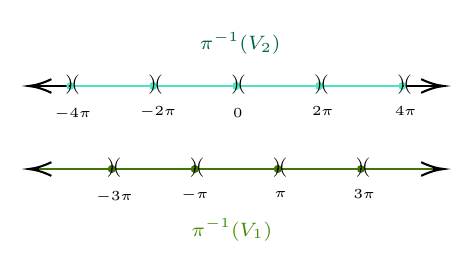
\begin{tikzpicture}[x=0.75pt,y=0.75pt,yscale=-1,xscale=1]
		%uncomment if require: \path (0,300); %set diagram left start at 0, and has height of 300
		
		%Straight Lines [id:da21155715150907928] 
		\draw    (102,100) -- (298,100) ;
		\draw [shift={(300,100)}, rotate = 180] [color={rgb, 255:red, 0; green, 0; blue, 0 }  ][line width=0.75]    (10.93,-3.29) .. controls (6.95,-1.4) and (3.31,-0.3) .. (0,0) .. controls (3.31,0.3) and (6.95,1.4) .. (10.93,3.29)   ;
		\draw [shift={(100,100)}, rotate = 0] [color={rgb, 255:red, 0; green, 0; blue, 0 }  ][line width=0.75]    (10.93,-3.29) .. controls (6.95,-1.4) and (3.31,-0.3) .. (0,0) .. controls (3.31,0.3) and (6.95,1.4) .. (10.93,3.29)   ;
		%Straight Lines [id:da6053815708812693] 
		\draw    (102,140) -- (298,140) ;
		\draw [shift={(300,140)}, rotate = 180] [color={rgb, 255:red, 0; green, 0; blue, 0 }  ][line width=0.75]    (10.93,-3.29) .. controls (6.95,-1.4) and (3.31,-0.3) .. (0,0) .. controls (3.31,0.3) and (6.95,1.4) .. (10.93,3.29)   ;
		\draw [shift={(100,140)}, rotate = 0] [color={rgb, 255:red, 0; green, 0; blue, 0 }  ][line width=0.75]    (10.93,-3.29) .. controls (6.95,-1.4) and (3.31,-0.3) .. (0,0) .. controls (3.31,0.3) and (6.95,1.4) .. (10.93,3.29)   ;
		%Straight Lines [id:da08565959039002635] 
		\draw [color={rgb, 255:red, 80; green, 227; blue, 194 }  ,draw opacity=1 ]   (160.34,100) -- (199.66,100) ;
		\draw [shift={(200,100)}, rotate = 0] [color={rgb, 255:red, 80; green, 227; blue, 194 }  ,draw opacity=1 ][line width=0.75]      (0, 0) circle [x radius= 1.34, y radius= 1.34]   ;
		\draw [shift={(160,100)}, rotate = 0] [color={rgb, 255:red, 80; green, 227; blue, 194 }  ,draw opacity=1 ][line width=0.75]      (0, 0) circle [x radius= 1.34, y radius= 1.34]   ;
		%Straight Lines [id:da27250605120330373] 
		\draw [color={rgb, 255:red, 80; green, 227; blue, 194 }  ,draw opacity=1 ]   (200.34,100) -- (239.66,100) ;
		\draw [shift={(240,100)}, rotate = 0] [color={rgb, 255:red, 80; green, 227; blue, 194 }  ,draw opacity=1 ][line width=0.75]      (0, 0) circle [x radius= 1.34, y radius= 1.34]   ;
		\draw [shift={(200,100)}, rotate = 0] [color={rgb, 255:red, 80; green, 227; blue, 194 }  ,draw opacity=1 ][line width=0.75]      (0, 0) circle [x radius= 1.34, y radius= 1.34]   ;
		%Straight Lines [id:da05693789649195624] 
		\draw [color={rgb, 255:red, 80; green, 227; blue, 194 }  ,draw opacity=1 ]   (240.34,100) -- (279.66,100) ;
		\draw [shift={(280,100)}, rotate = 0] [color={rgb, 255:red, 80; green, 227; blue, 194 }  ,draw opacity=1 ][line width=0.75]      (0, 0) circle [x radius= 1.34, y radius= 1.34]   ;
		\draw [shift={(240,100)}, rotate = 0] [color={rgb, 255:red, 80; green, 227; blue, 194 }  ,draw opacity=1 ][line width=0.75]      (0, 0) circle [x radius= 1.34, y radius= 1.34]   ;
		%Straight Lines [id:da8842492506901922] 
		\draw [color={rgb, 255:red, 80; green, 227; blue, 194 }  ,draw opacity=1 ]   (120.34,100) -- (159.66,100) ;
		\draw [shift={(160,100)}, rotate = 0] [color={rgb, 255:red, 80; green, 227; blue, 194 }  ,draw opacity=1 ][line width=0.75]      (0, 0) circle [x radius= 1.34, y radius= 1.34]   ;
		\draw [shift={(120,100)}, rotate = 0] [color={rgb, 255:red, 80; green, 227; blue, 194 }  ,draw opacity=1 ][line width=0.75]      (0, 0) circle [x radius= 1.34, y radius= 1.34]   ;
		%Straight Lines [id:da40037042015505686] 
		\draw [color={rgb, 255:red, 65; green, 117; blue, 5 }  ,draw opacity=1 ]   (220.34,140) -- (259.66,140) ;
		\draw [shift={(260,140)}, rotate = 0] [color={rgb, 255:red, 65; green, 117; blue, 5 }  ,draw opacity=1 ][line width=0.75]      (0, 0) circle [x radius= 1.34, y radius= 1.34]   ;
		\draw [shift={(220,140)}, rotate = 0] [color={rgb, 255:red, 65; green, 117; blue, 5 }  ,draw opacity=1 ][line width=0.75]      (0, 0) circle [x radius= 1.34, y radius= 1.34]   ;
		%Straight Lines [id:da8428207291783898] 
		\draw [color={rgb, 255:red, 65; green, 117; blue, 5 }  ,draw opacity=1 ]   (180.34,140) -- (219.66,140) ;
		\draw [shift={(220,140)}, rotate = 0] [color={rgb, 255:red, 65; green, 117; blue, 5 }  ,draw opacity=1 ][line width=0.75]      (0, 0) circle [x radius= 1.34, y radius= 1.34]   ;
		\draw [shift={(180,140)}, rotate = 0] [color={rgb, 255:red, 65; green, 117; blue, 5 }  ,draw opacity=1 ][line width=0.75]      (0, 0) circle [x radius= 1.34, y radius= 1.34]   ;
		%Straight Lines [id:da49958094115942586] 
		\draw [color={rgb, 255:red, 65; green, 117; blue, 5 }  ,draw opacity=1 ]   (140.34,140) -- (179.66,140) ;
		\draw [shift={(180,140)}, rotate = 0] [color={rgb, 255:red, 65; green, 117; blue, 5 }  ,draw opacity=1 ][line width=0.75]      (0, 0) circle [x radius= 1.34, y radius= 1.34]   ;
		\draw [shift={(140,140)}, rotate = 0] [color={rgb, 255:red, 65; green, 117; blue, 5 }  ,draw opacity=1 ][line width=0.75]      (0, 0) circle [x radius= 1.34, y radius= 1.34]   ;
		%Straight Lines [id:da8644029227526777] 
		\draw [color={rgb, 255:red, 65; green, 117; blue, 5 }  ,draw opacity=1 ]   (105,140) -- (139.66,140) ;
		\draw [shift={(140,140)}, rotate = 0] [color={rgb, 255:red, 65; green, 117; blue, 5 }  ,draw opacity=1 ][line width=0.75]      (0, 0) circle [x radius= 1.34, y radius= 1.34]   ;
		%Straight Lines [id:da08267172889438279] 
		\draw [color={rgb, 255:red, 65; green, 117; blue, 5 }  ,draw opacity=1 ]   (260,140) -- (295,140) ;
		
		% Text Node
		\draw (199,93.4) node [anchor=north west][inner sep=0.75pt]  [font=\scriptsize]  {$($};
		% Text Node
		\draw (239,93.4) node [anchor=north west][inner sep=0.75pt]  [font=\scriptsize]  {$($};
		% Text Node
		\draw (279,93.4) node [anchor=north west][inner sep=0.75pt]  [font=\scriptsize]  {$($};
		% Text Node
		\draw (159,93.4) node [anchor=north west][inner sep=0.75pt]  [font=\scriptsize]  {$($};
		% Text Node
		\draw (119,93.4) node [anchor=north west][inner sep=0.75pt]  [font=\scriptsize]  {$($};
		% Text Node
		\draw (116,93.4) node [anchor=north west][inner sep=0.75pt]  [font=\scriptsize]  {$)$};
		% Text Node
		\draw (156,93.4) node [anchor=north west][inner sep=0.75pt]  [font=\scriptsize]  {$)$};
		% Text Node
		\draw (196,93.4) node [anchor=north west][inner sep=0.75pt]  [font=\scriptsize]  {$)$};
		% Text Node
		\draw (236,93.4) node [anchor=north west][inner sep=0.75pt]  [font=\scriptsize]  {$)$};
		% Text Node
		\draw (276,93.4) node [anchor=north west][inner sep=0.75pt]  [font=\scriptsize]  {$)$};
		% Text Node
		\draw (197,109.4) node [anchor=north west][inner sep=0.75pt]  [font=\tiny]  {$0$};
		% Text Node
		\draw (235,108.4) node [anchor=north west][inner sep=0.75pt]  [font=\tiny]  {$2\pi $};
		% Text Node
		\draw (275,108.4) node [anchor=north west][inner sep=0.75pt]  [font=\tiny]  {$4\pi $};
		% Text Node
		\draw (152,108.4) node [anchor=north west][inner sep=0.75pt]  [font=\tiny]  {$-2\pi $};
		% Text Node
		\draw (111,109.4) node [anchor=north west][inner sep=0.75pt]  [font=\tiny]  {$-4\pi $};
		% Text Node
		\draw (219,133.4) node [anchor=north west][inner sep=0.75pt]  [font=\scriptsize]  {$($};
		% Text Node
		\draw (259,133.4) node [anchor=north west][inner sep=0.75pt]  [font=\scriptsize]  {$($};
		% Text Node
		\draw (179,133.4) node [anchor=north west][inner sep=0.75pt]  [font=\scriptsize]  {$($};
		% Text Node
		\draw (139,133.4) node [anchor=north west][inner sep=0.75pt]  [font=\scriptsize]  {$($};
		% Text Node
		\draw (136,133.4) node [anchor=north west][inner sep=0.75pt]  [font=\scriptsize]  {$)$};
		% Text Node
		\draw (176,133.4) node [anchor=north west][inner sep=0.75pt]  [font=\scriptsize]  {$)$};
		% Text Node
		\draw (216,133.4) node [anchor=north west][inner sep=0.75pt]  [font=\scriptsize]  {$)$};
		% Text Node
		\draw (256,133.4) node [anchor=north west][inner sep=0.75pt]  [font=\scriptsize]  {$)$};
		% Text Node
		\draw (217,149.4) node [anchor=north west][inner sep=0.75pt]  [font=\tiny]  {$\pi $};
		% Text Node
		\draw (255,148.4) node [anchor=north west][inner sep=0.75pt]  [font=\tiny]  {$3\pi $};
		% Text Node
		\draw (172,148.4) node [anchor=north west][inner sep=0.75pt]  [font=\tiny]  {$-\pi $};
		% Text Node
		\draw (131,149.4) node [anchor=north west][inner sep=0.75pt]  [font=\tiny]  {$-3\pi $};
		% Text Node
		\draw (181,72.4) node [anchor=north west][inner sep=0.75pt]  [font=\scriptsize,color={rgb, 255:red, 0; green, 97; blue, 73 }  ,opacity=1 ]  {$\pi ^{-1}( V_{2})$};
		% Text Node
		\draw (177,162.4) node [anchor=north west][inner sep=0.75pt]  [font=\scriptsize,color={rgb, 255:red, 70; green, 139; blue, 5 }  ,opacity=1 ]  {$\pi ^{-1}( V_{1})$};
		
		
	\end{tikzpicture}
\end{figure}
		On the other hand we have
		\begin{align*}
			&U_1\cap \inv{\bar{\phi}}(V_1) = (\inv{\phi_1}\circ\inv{\pi})(V_1),  
			\quad U_2\cap \inv{\bar{\phi}}(V_1) = (\inv{\phi_2}\circ\inv{\pi})(V_1),\\
			\quad &U_1\cap \inv{\bar{\phi}}(V_2) = (\inv{\phi_1}\circ\inv{\pi})(V_2),
			\quad U_2\cap \inv{\bar{\phi}}(V_2) = (\inv{\phi_2}\circ\inv{\pi})(V_2).
		\end{align*}
		The image of these maps are shown in the figure below
		\begin{figure}[h!]
	\centering
	
	
	
	\tikzset{every picture/.style={line width=0.75pt}} %set default line width to 0.75pt        
	
	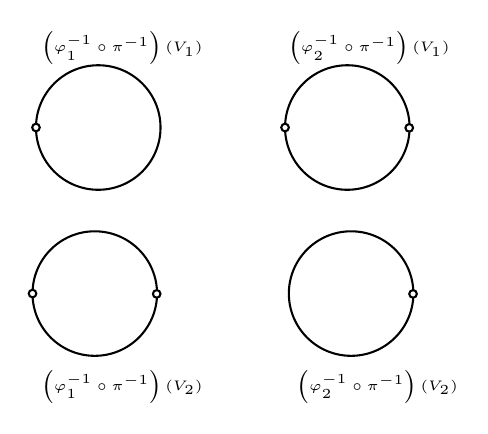
\begin{tikzpicture}[x=0.75pt,y=0.75pt,yscale=-1,xscale=1]
		%uncomment if require: \path (0,300); %set diagram left start at 0, and has height of 300
		
		%Shape: Circle [id:dp7624927902795768] 
		\draw   (90,80) .. controls (90,63.43) and (103.43,50) .. (120,50) .. controls (136.57,50) and (150,63.43) .. (150,80) .. controls (150,96.57) and (136.57,110) .. (120,110) .. controls (103.43,110) and (90,96.57) .. (90,80) -- cycle ;
		%Shape: Circle [id:dp8279394743167126] 
		\draw  [fill={rgb, 255:red, 255; green, 255; blue, 255 }  ,fill opacity=1 ] (88.17,80) .. controls (88.17,78.99) and (88.99,78.17) .. (90,78.17) .. controls (91.01,78.17) and (91.83,78.99) .. (91.83,80) .. controls (91.83,81.01) and (91.01,81.83) .. (90,81.83) .. controls (88.99,81.83) and (88.17,81.01) .. (88.17,80) -- cycle ;
		%Shape: Circle [id:dp9009991128602786] 
		\draw   (210,80) .. controls (210,63.43) and (223.43,50) .. (240,50) .. controls (256.57,50) and (270,63.43) .. (270,80) .. controls (270,96.57) and (256.57,110) .. (240,110) .. controls (223.43,110) and (210,96.57) .. (210,80) -- cycle ;
		%Shape: Circle [id:dp06103467761022641] 
		\draw  [fill={rgb, 255:red, 255; green, 255; blue, 255 }  ,fill opacity=1 ] (208.17,80) .. controls (208.17,78.99) and (208.99,78.17) .. (210,78.17) .. controls (211.01,78.17) and (211.83,78.99) .. (211.83,80) .. controls (211.83,81.01) and (211.01,81.83) .. (210,81.83) .. controls (208.99,81.83) and (208.17,81.01) .. (208.17,80) -- cycle ;
		%Shape: Circle [id:dp10180676331611016] 
		\draw  [fill={rgb, 255:red, 255; green, 255; blue, 255 }  ,fill opacity=1 ] (268,80.17) .. controls (268,79.15) and (268.82,78.33) .. (269.83,78.33) .. controls (270.85,78.33) and (271.67,79.15) .. (271.67,80.17) .. controls (271.67,81.18) and (270.85,82) .. (269.83,82) .. controls (268.82,82) and (268,81.18) .. (268,80.17) -- cycle ;
		%Shape: Circle [id:dp855196723421777] 
		\draw   (88.33,160) .. controls (88.33,143.43) and (101.76,130) .. (118.33,130) .. controls (134.9,130) and (148.33,143.43) .. (148.33,160) .. controls (148.33,176.57) and (134.9,190) .. (118.33,190) .. controls (101.76,190) and (88.33,176.57) .. (88.33,160) -- cycle ;
		%Shape: Circle [id:dp4627947669837389] 
		\draw  [fill={rgb, 255:red, 255; green, 255; blue, 255 }  ,fill opacity=1 ] (86.5,160) .. controls (86.5,158.99) and (87.32,158.17) .. (88.33,158.17) .. controls (89.35,158.17) and (90.17,158.99) .. (90.17,160) .. controls (90.17,161.01) and (89.35,161.83) .. (88.33,161.83) .. controls (87.32,161.83) and (86.5,161.01) .. (86.5,160) -- cycle ;
		%Shape: Circle [id:dp14067791390529916] 
		\draw  [fill={rgb, 255:red, 255; green, 255; blue, 255 }  ,fill opacity=1 ] (146.33,160.17) .. controls (146.33,159.15) and (147.15,158.33) .. (148.17,158.33) .. controls (149.18,158.33) and (150,159.15) .. (150,160.17) .. controls (150,161.18) and (149.18,162) .. (148.17,162) .. controls (147.15,162) and (146.33,161.18) .. (146.33,160.17) -- cycle ;
		%Shape: Circle [id:dp4395956628276514] 
		\draw   (211.83,160) .. controls (211.83,143.43) and (225.26,130) .. (241.83,130) .. controls (258.4,130) and (271.83,143.43) .. (271.83,160) .. controls (271.83,176.57) and (258.4,190) .. (241.83,190) .. controls (225.26,190) and (211.83,176.57) .. (211.83,160) -- cycle ;
		%Shape: Circle [id:dp3289592382066828] 
		\draw  [fill={rgb, 255:red, 255; green, 255; blue, 255 }  ,fill opacity=1 ] (269.83,160.17) .. controls (269.83,159.15) and (270.65,158.33) .. (271.67,158.33) .. controls (272.68,158.33) and (273.5,159.15) .. (273.5,160.17) .. controls (273.5,161.18) and (272.68,162) .. (271.67,162) .. controls (270.65,162) and (269.83,161.18) .. (269.83,160.17) -- cycle ;
		
		% Text Node
		\draw (91,32.4) node [anchor=north west][inner sep=0.75pt]  [font=\tiny]  {$\left( \varphi _{1}^{-1} \circ \pi ^{-1}\right)( V_{1})$};
		% Text Node
		\draw (210,32.4) node [anchor=north west][inner sep=0.75pt]  [font=\tiny]  {$\left( \varphi _{2}^{-1} \circ \pi ^{-1}\right)( V_{1})$};
		% Text Node
		\draw (91,195.4) node [anchor=north west][inner sep=0.75pt]  [font=\tiny]  {$\left( \varphi _{1}^{-1} \circ \pi ^{-1}\right)( V_{2})$};
		% Text Node
		\draw (214,195.4) node [anchor=north west][inner sep=0.75pt]  [font=\tiny]  {$\left( \varphi _{2}^{-1} \circ \pi ^{-1}\right)( V_{2})$};
		
		
	\end{tikzpicture}
\end{figure}
		\FloatBarrier
		Thus we will have
		\begin{align*}
			&\phi_1(U_1\cap \inv{\bar{\phi}}(V_1)) = (-\pi,\pi),\\
			&\phi_2(U_2\cap \inv{\bar{\phi}}(V_1)) = (0,\pi)\cup(\pi,2\pi),\\
			&\phi_1(U_1\cap \inv{\bar{\phi}}(V_2)) = (-\pi,0) \cup (0,\pi),\\
			&\phi_2(U_2\cap \inv{\bar{\phi}}(V_2)) = (0,2\pi).
		\end{align*}
		
		Now we can re-write the maps of interest as
		\begin{align*}
			&\psi_1\circ\bar{\phi}\circ\inv{\phi_1}: (-\pi,\pi)\to \psi_1(\bar{\phi}(U_1)),\\
			&\psi_1\circ\bar{\phi}\circ\inv{\phi_2}:(0,\pi)\cup(\pi,2\pi)\to \psi_1(\bar{\phi}(U_2)),\\
			&\psi_2\circ\bar{\phi}\circ\inv{\phi_1}: (-\pi,0) \cup (0,\pi)\to \psi_2(\bar{\phi}(U_1)),\\
			&\psi_2\circ\bar{\phi}\circ\inv{\phi_2}: (0,2\pi)\to \psi_2(\bar{\phi}(U_2)).
		\end{align*}
		which are given by
		\begin{align*}
			&(\psi_1\circ\bar{\phi}\circ\inv{\phi_1})(t) = (\psi_1\circ(\pi\circ\phi_1)\circ\inv{\phi_1})(t) = \psi_1(\pi(t)) = \psi_1([t]) = t, \qquad t \in (-\pi,\pi).\\
			&(\psi_1\circ\bar{\phi}\circ\inv{\phi_2})(t) = (\psi_1\circ(\pi\circ\phi_2)\circ\inv{\phi_2})(t) = \psi_1(\pi(t)) = \phi_1([t]) = \begin{cases}
				t \qquad & t\in (0,\pi),\\
				t-2\pi \qquad & t\in (\pi,2\pi).
			\end{cases}\\
			&(\psi_2\circ\bar{\phi}\circ\inv{\phi_1})(t) = (\psi_2\circ(\pi\circ\phi)\circ\inv{\phi_1})(t) = \psi_2(\pi(t)) = \psi_2([t]) = \begin{cases}
				t+2\pi \qquad & t \in (-\pi,0),\\
				t \qquad & t\in (0,\pi).
			\end{cases}\\
			&(\psi_2\circ\bar{\phi}\circ\inv{\phi_2})(t) = (\psi_2\circ(\pi\circ\phi_2)\circ\inv{\phi_2})(t) = \psi_2(\pi(t)) = \psi_2(t) = t, \qquad t \in (0,2\pi).
		\end{align*}
		All of the maps above are $ C^\infty $. This shows that $ \bar{\psi} $ is indeed $ C^\infty $.
		
		\item With a similar approach as above, using \autoref{def:SmoothMapsBetweenManifolds} we need to show that the following maps are smooth.
		\begin{align*}
			&\phi_1\circ F\circ \inv{\psi_1}:\psi_1(V_1\cap \inv{F}(U_1)) \to \phi_1(F(U_1))\\
			&\phi_1\circ F\circ \inv{\psi_2}:\psi_2(V_2\cap \inv{F}(U_1)) \to \phi_1(F(U_2)) \\
			&\phi_2\circ F\circ \inv{\psi_1}:\psi_1(V_1\cap \inv{F}(U_2)) \to \phi_2(F(U_1))\\
			&\phi_2\circ F\circ \inv{\psi_2}:\psi_2(V_2\cap \inv{F}(U_2)) \to \phi_2(F(U_2))
		\end{align*}
		First, observe that
		\begin{align*}
			&V_1 \cap \inv{F}(U_1) = \set{[t]\ |\ t\in (-\pi,\pi)} \implies \psi_1(V_1 \cap \inv{F}(U_1)) = (-\pi,\pi), 
			\\
			&V_2 \cap \inv{F}(U_1) = \set{[t]\ |\ t\in (0,\pi)\cup(\pi,2\pi)} \implies  \psi_2(V_2 \cap \inv{F}(U_1)) = (0,\pi)\cup(\pi,2\pi),
			\\
			&V_1\cap\inv{F}(U_2) = \set{[t]\ |\ t\in (-\pi,0)\cup(0,\pi)} \implies \psi_1(V_1\cap\inv{F}(U_2)) = (-\pi,0)\cup(0,\pi), 
			\\
			&V_2\cap\inv{F}(U_2) = \set{[t]\ |\ t\in (0,2\pi)} \implies \psi_2(V_2\cap\inv{F}(U_2)) = (0,2\pi).
		\end{align*}
		Thus we can re-write the map definitions
		\begin{align*}
			&\phi_1\circ F\circ \inv{\psi_1}:(-\pi,\pi) \to \phi_1(F(U_1))\\
			&\phi_1\circ F\circ \inv{\psi_2}:(0,\pi)\cup(\pi,2\pi) \to \phi_1(F(U_2)) \\
			&\phi_2\circ F\circ \inv{\psi_1}:(-\pi,0)\cup(0,\pi) \to \phi_2(F(U_1))\\
			&\phi_2\circ F\circ \inv{\psi_2}:(0,2\pi) \to \phi_2(F(U_2))
		\end{align*}
		These maps are given by
		\begin{align*}
			&(\phi_1\circ F\circ \inv{\psi_1})(t) = \phi_1(e^{it}) = t, \qquad t\in(-\pi,\pi) .\\
			&(\phi_1\circ F\circ \inv{\psi_2})(t) = \begin{cases}
				t \qquad & t\in (0,\pi),\\
				t -2\pi & t\in (\pi,2\pi).
			\end{cases}\\
			&(\phi_2\circ F\circ \inv{\psi_1})(t) = \begin{cases}
				t + 2\pi \qquad & t\in (-\pi,0),\\
				t \qquad & t\in (0,\pi).
			\end{cases}\\
			&(\phi_2\circ F\circ \inv{\psi_2})(t) = \phi_2(e^{it}) = t, \qquad t\in(-\pi,\pi).
		\end{align*}
		All of the functions above are $ C^\infty $. Thus $ F $ is $ C^\infty $.
		
		\item To show that $ F:\R/2\pi\Z \to S^1 $ is a diffeomorphism it is enough to show that $ \bar{\phi} : S^1 \to \R/2\pi\Z $ is inverse of it. Consider the following composition of maps
		\[ F\circ\bar{\phi}: S^1 \to S^1. \]
		For the points $ x \in U_1 \subset S^1 $, since $ U_1 = \set{e^{it}\ |\ t\in(-\pi,\pi)} $ we have
		\[ (F\circ\pi\circ\phi_1)(x) = (F\circ\pi\circ\phi_1)(\underbrace{e^{it}}_{t\in(-\pi,\pi)}) = (F(\pi(t))) = F([t]) = e^{it}.  \]
		Similarly, for the points $ x \in U_2 \subset S^1 $, since $ U_2 = \set{e^{it}\ |\ t \in (0,2\pi)} $ we have 
		\[ (F\circ\pi\circ\phi_2)(x) = (F\circ\pi\circ\phi_2)(\underbrace{e^{it}}_{t\in(0,2\pi)}) = F(\pi(t)) = F([t]) = e^{it}. \]
		For the converse, consider the following map
		\[ \bar{\phi}\circ F : \R/2\pi\Z \to \R/2\pi\Z. \]
		Let $ [t] \in \R/2\pi\Z $. Then we have
		\[ (\bar{\phi}\circ F)([t]) = \bar{\phi}(e^{it}) = \pi(t + 2n\pi)  = [t] \qquad \text{for some $ n\in \Z $}. \]
		This shows that $ F $ is indeed a diffeomorphism between manifolds.
	\end{enumerate}
	\begin{summary}
		In the question above, we proved (by finding an explicit diffeomorphism) that $ \R/2\pi\Z $ is diffeomorphic to $ S^1 \subset \C $.
	\end{summary}
\end{solution}

\begin{problem}[The Grassmannian $ G(k,n) $]
	\label{problem:Grassmannian}
	The Grassmannian $ G(k,n) $ is the set of all $ k\text{-planes} $ through the origin in $ \R^n $. Such a $ k\text{-plane} $ is a linear subspace of dimension $ k $ of $ \R^n $ and has a basis consisting of $ k $ linearly independent vectors $ a_1,\cdots,a_k $ in $ \R^n $. IT is therefore completely specified by an $ n\times k $ matrix $ A = [a_1\ \cdots\ a_k] $ of rank $ k $, where the rank of a matrix $ A $, denoted by $ \rank A $ is defined to be the number of linearly independent columns of $ A $. This matrix is called a matrix representative of the $ k\text{-plane} $.
	
	Two bases $ a_1,\cdots,a_k $ and $ b_1,\cdots,b_k $ determine the same $ k\text{-planes} $ if there is a change of basis matrix $ g = [g_{ij}] \in GL(k,\R) $ such that 
	\[ \vecttt{b_1}{\vdots}{b_k} = g^T \vecttt{a_1}{\vdots}{a_k}, \]
	or equivalently
	\[ b_j = \sum_{i}g_{ij}a_j, \]
	or in matrix notation
	\[ B = Ag \]
	where $ B,A $ are matrices whose columns are the vectors $ a_1,\cdots,a_k $ and $ b_1,\cdots,b_k $ respectively.
	
	Let $ F(k,n) $ denote the set of all $ n\times k $ matrices of rank $ k $, topologized as a subspace of $ R^{n\times k} $. Thus $ F(k,n) $ is an open subset of $ R^{n\times k} $.
	
	Let the group $ GL(k,\R) $ act on $ F(k,n) $ on the right by $ A\cdot g = Ag $ where the right hand side is the usual matrix multiplication. Consider the orbit space $ F(k,n)/GL(k,\R) $. Equivalently, we can show this space as the quotient space $ F(k,n)/\sim $ where the equivalence relation $ \sim $ is given as
	\[ A \equiv B \qquad \text{iff} \qquad A = Bg \quad \text{for some $ g \in GL(n,\R) $}. \]
	There is a bijection between the Grassmannian $ G(k,n) $  and the orbit space $ f(k,n)/GL(k,\R) $. We given the Grassmannian $ G(k,n) $ the quotient topology on $ F(k,n)/GL $.
	\begin{enumerate}[(a)]
		\item Show that $ \sim $ is an open equivalence relation.
		\item Prove that the Grassmannian $ G(k,n) $ is second countable.
		\item Let $ S = F(k,n) $. Prove that the graph $ R $ in $ S\times S $ of the equivalence relation $ \sim $ is closed. (\emph{Hint}: Two matrices $ A = [a_1\ \cdots\ a_k]$ and $ B = [b_1\ \cdots\ b_k] $ are equivalent $ \Leftrightarrow $ every column of $ B $ is a linear combination of the columns of $ A $ $ \Leftrightarrow $ $ \rank[A\ B] \leq k $ $ \Leftrightarrow $ all $ (k+1)\times(k+1) $ minors of $ [A\ B] $ are zero).
		\item Prove that the Grassmannian $ G(n,k) $ is Hausdorff.
		
		Now we want to find a $ C^\infty $ atlas on the Grassmannian $ G(k,n) $. For simplicity, we specialize to $ G(2,4) $. For any $ 4\times 2 $ matrix $ A $, let $ A_{ij} $ be the $ 2\times 2 $ sub matrix consisting of its $ i\text{th} $ row and $ j\text{th} $ row. Define
		\[ V_{ij} = \set{A \in F(2,4)\ |\ A_{ij} \text{ is nonsingular}}. \]
		For any $ A \in V_{ij} $, since $ \det(A_{ij}) \neq 0 $ (i.e. it is nonsingular), then we can perturb it small enough and by continuoity of the determinant operator the nonsingularity of $ A_{ij} $ persists. This shows that $ V_{ij} $ is indeed an open subset of $ F(2,4) $. Alternatively, we can show this by arguing that since the complement of $ V_{ij} $ is defined by vanishing of $ \det(A_{ij}) $, we conclude that $ V_{ij} $ is an open subset of $ F(2,4) $.
		
		\item Prove that if $ A \in V_{ij} $, then $ Ag \in V_{ij} $ for any nonsingular matrix $ g \in GL(2,\R) $.
		
		Define $ U_{ij} = V_{ij}/\sim $. Since $ \sim $ is an open equivalence relation, $ U_{ij}$ is an open subset of $ G(2,4) $. For $ A \in V_{12} $
		\[ A \sim A \inv{A}_{12} = 
		\begin{bmatrix}
			1 & 0 \\
			0 & 1 \\
			\ast & \ast \\
			\ast & \ast 
		\end{bmatrix} = 
		\begin{bmatrix}
			I \\
			A_{34}\inv{A}_{12}
		\end{bmatrix}.
		 \]
		 This shows that the matrix representative of a $ 2\text{-plane} $ in $ U_{12} $ have a canonical form $ B $ where $ B_{12} $ is the identity matrix.
		 
		 \item Show that the map $ \tilde{\phi}_{12}: V_{12} \to \R^{2\times 2} $,
		 \[ \tilde{\phi}_{12} (A) = A_{34}\inv{A}_{12} \]
		 induces a homeomorphism $ \phi_{12}: U_{12} \to \R{2\times 2} $.
		
	\end{enumerate}

		
\end{problem}

\begin{solution}
			$ \ $
	\begin{enumerate}[(a)]
		\item According to \autoref{lemma:contGroupActionOpenProjection} the projection map $ \pi : F(k,n) \to F(k,n)/GL $ is an open map if and only if the group action map $ \alpha:  F(k,n)\times G \to  F(k,n)  $ is continuous. Let $ A \in F(k,n) $ and $ g \in G $. Then $ B = \alpha(A,g) $. For the element $ b_{kl} $ of $ B $ we have 
		\[ b_{kl} = \sum_{i} A_{ki}g_{il} \]
		which is a polynomial. Thus $ \alpha $ is a continuous map. Now according to \autoref{lemma:contGroupActionOpenProjection} the equivalence relation $ \sim $ is open.
		
		\item From \autoref{prop:secondCountalbeQuotientSpace} it follows that since $ \sim $ is an open equivalence relation, then quotient space $ G(k,n) = F(k,n)/\sim $ is second countable.
		
		\item To show that $ R $ is closed by showing that it complement is open. Let $ x \in R^c $. Then $ x = [A\ B] $ for some matrices $ A,B \in S $ where the matrix $ [A\ B] $ has at least on $ (k+1)\times (k+1) $ that is not zero. Then by continuoity of determinant operation, for small enough $ \epsilon >0 $ we can find an open ball $ \mathbb{B}_\epsilon $ centered at $ [A\ B] \in \R^{n\times2k}$ such that for all $ y \in \mathbb{B}_\epsilon  $ the non-zero minor persists. This shows that $ R^c $ is open which implies the closedness of $ R $.
		
		\item Since $ \sim $ is an open equivalence relation and also the graph of the equivalence relation is closed in $ S\times S $, then by \autoref{thm:QuotientIsHausdorff} it follows that $ G(k,n) $ is Hausdorff.
		
		\item First, observe that 
		\[ (Ag)_{ij} = A_{ij} g. \]
		Let $ A \in V_{ij} $. Then from definition we know that $ \det(A_{ij}) \neq 0 $. Since $ (Ag)_{ij} = A_{ij}g $ and $ \det((Ag)_{ij}) = \det(A_{ij})\det(g) $, then from nonsingularity of $ g $ it follows that $ \det((Ag)_{ij}) \neq 0 $. Hence $ Ag \in V_{ij} $.
		
		\item Consider the following diagram.
		% https://q.uiver.app/#q=WzAsMyxbMCwwLCJWX3sxMn0iXSxbMCwxLCJVX3sxMn0iXSxbMSwwLCJcXFJeezJcXHRpbWVzIDJ9Il0sWzAsMSwiXFxwaSIsMl0sWzAsMiwiXFx0aWxkZXtcXHBoaX1fezEyfSJdLFsxLDIsIlxccGhpX3sxMn0iLDJdXQ==
		\[\begin{tikzcd}
			{V_{12}} & {\R^{2\times 2}} \\
			{U_{12}}
			\arrow["{\tilde{\phi}_{12}}", from=1-1, to=1-2]
			\arrow["\pi"', from=1-1, to=2-1]
			\arrow["{\phi_{12}}"', from=2-1, to=1-2]
		\end{tikzcd}\]
		First observe that $ \tilde{\phi}_{12} $ assumes a constant value for all the points in its domain that are in the same equivalence class. That is because if for $ A,B \in V_{12} $ we have $ A\sim B $, then $ \exists g \in GL(2,\R) $ such that $ A = Bg $. Thus
		\[ A_{34}\inv{A}_{12} = \tilde{\phi}_{12} (A) = \tilde{\phi}_{12}(Bg) = (Bg)_{34}\inv{(Bg)}_{12} = B_{34}g \inv{g}\inv{B}_{12} = B_{34}\inv{B}_{12}. \]
		Also, since $ \tilde{\phi}_{12} $ is continuous, then it follows that the induced map $ \phi_{12} $ is also continuous.
		
		Now, we need to find an inverse for this map. Consider the map
		\[ \psi_{12} : \R^{2\times 2} \to U_{12}, \ M \mapsto \vectt{I}{M}. \]
		This inclusion map is indeed continuous. Now we need to show that $ \psi $ and $ \phi $ are inverse maps. Consider 
		\[ \psi\circ{\phi} : U_{12} \to U_{12}. \]
		Let $ A \in U_{12} $. Then we know that there exist a canonical representation of $ A $ as 
		\[ A \ \sim \vectt{I}{A_{34}\inv{A}_{12}}. \]
		Then 
		\[ \psi(\phi( \vectt{I}{A_{34}\inv{A}_{12}})) = \psi(A_{34}\inv{A}_{12}) = \vectt{I}{A_{34}\inv{A}_{12}} \]
		For the converse, consider the map
		\[ \phi\circ{\psi}: R^{2\times 2}\to \R^{2\times 2}. \]
		Let $ M \in \R^{2\times 2} $. Then 
		\[ (\phi\circ{\psi})(M) = \phi(\vectt{I}{M}) = M.  \]
		This shows that $ \psi $ and $ \phi $ are inverse maps and this completes the proof.
		
		
	\end{enumerate}
	
\end{solution}

\newpage
